% Origen: Secciones/PI - Implementacion MCA.md
% El "Apéndice" de la nota va en apend7.tex (Detalles del MCA). Lo que en la nota
% está entre %% (datapath del trapecio, funcionamiento interno del conformado,
% criterio de separación, elección de parámetros) no se transcribe.
\chapter{Implementación del MCA}
\label{C:implmca}

% Figuras de ESTE capítulo + las compartidas. Siempre al principio del archivo.
\graphicspath{{figs/cap7/}{figs/comunes/}}

\begin{destacado}
En este capítulo describimos (1) las funcionalidades ofrecidas por el módulo
MCA, (2) su método de utilización desde el PS, (3) una vista general del módulo
a nivel de HW, (4) el análisis del tiempo muerto y de los eventos perdidos, (5)
los métodos de recuperación del pulso y (6) los detalles de implementación de
cada submódulo. En el apéndice se presentan la detección del solape, la primera
versión del módulo, la elección de la cantidad de canales y el mapa de
registros. En el Cap.~\ref{C:resultados} se presentan las figuras de mérito
medidas para este módulo.
\end{destacado}

Este módulo tiene como entrada el flujo de muestras de los dos canales de
adquisición, ya calibradas y filtradas por el osciloscopio, y tres señales del
multitrigger (MT): el disparo \codigo{trig\_i}, que marca el comienzo de cada
evento, el veto \codigo{veto\_i} y el estado de re-armado del disparo,
\codigo{trig\_arm\_i}. Provee las siguientes funcionalidades:
\begin{itemize}
  \item \textbf{Histogramas de \emph{features} 1D y 2D}: un espectro de 8192 canales y
    un mapa de $128 \times 64$ bines. La cantidad de bines se fija en la
    síntesis; por registro se elige qué \emph{feature} va a cada eje y qué rango de
    ella cubre (\emph{zoom}).
  \item \textbf{Once \emph{features} por evento}, calculadas a la vez sobre el mismo
    pulso: pico, integral, dos de forma, la altura del conformado trapezoidal,
    y los tiempos y las marcas de solape con los pulsos vecinos
    (Tabla~\ref{t:implmca-estimadores}).
  \item \textbf{Medición de hasta \codigo{N\_ACC} eventos simultáneos}, cada uno
    en su ranura. El \emph{bitstream} trae \codigo{N\_ACC = 3}, y el registro
    \codigo{cfg\_n\_acc} elige cuántas se usan.
  \item \textbf{Banco de conformados trapezoidales} con corrección polo-cero:
    cada evento se publica con la forma más larga que sus vecinos permiten.
  \item \textbf{Línea de base} fija o con seguidor IIR.
  \item \textbf{Rechazo por criterios configurables}: una ventana de amplitud
    (sobre el pico o la integral) al cerrar cada evento, y un discriminador que
    acepta los eventos con una \emph{feature} elegida dentro, o fuera, de un
    intervalo.
  \item \textbf{Reporte del tiempo muerto y de los eventos perdidos}: el tiempo
    de adquisición desglosado por causa, la ocupación de las ranuras, tres
    estadísticos de los períodos muertos y un contador en cada punto donde se
    pierde o se rechaza un evento.
\end{itemize}

El criterio de finalización de eventos no se elige: la ventana la abre siempre
el disparo del MT y la cierra una compuerta fija. El cierre por histéresis se
retiró al pasar a medir varios pulsos a la vez, porque con ventanas superpuestas el
cruce de bajada es el de la señal sumada y cerraría todas juntas.

%==============================================================================
\section{Flujo de utilización del módulo}
\label{S:implmca-flujo}

En la Fig.~\ref{f:implmca-secuencia} se presenta el flujo de utilización.
Empieza con una \textbf{fase de configuración}, con \codigo{run = 0}, que se
realiza mediante el bus \emph{custom} de Pitaya. A continuación se usan los comandos de
control de la adquisición; en la figura se presenta la secuencia limpieza,
arranque, parada y lectura. Después de la limpieza (\codigo{CTRL.clear})
esperamos \codigo{clear\_busy = 0}, que indica que terminó el barrido de borrado
de los histogramas, y recién entonces arrancamos. Para leer, paramos con
\codigo{CTRL.run = 0} y esperamos \codigo{busy = 0}. Sin esa espera los valores
leídos no son estables: \codigo{run = 0} impide abrir ventanas nuevas, pero las
que estaban abiertas terminan de medir y el publicador sigue actualizando las
cuentas del histograma.

\begin{figure}[H]
\centering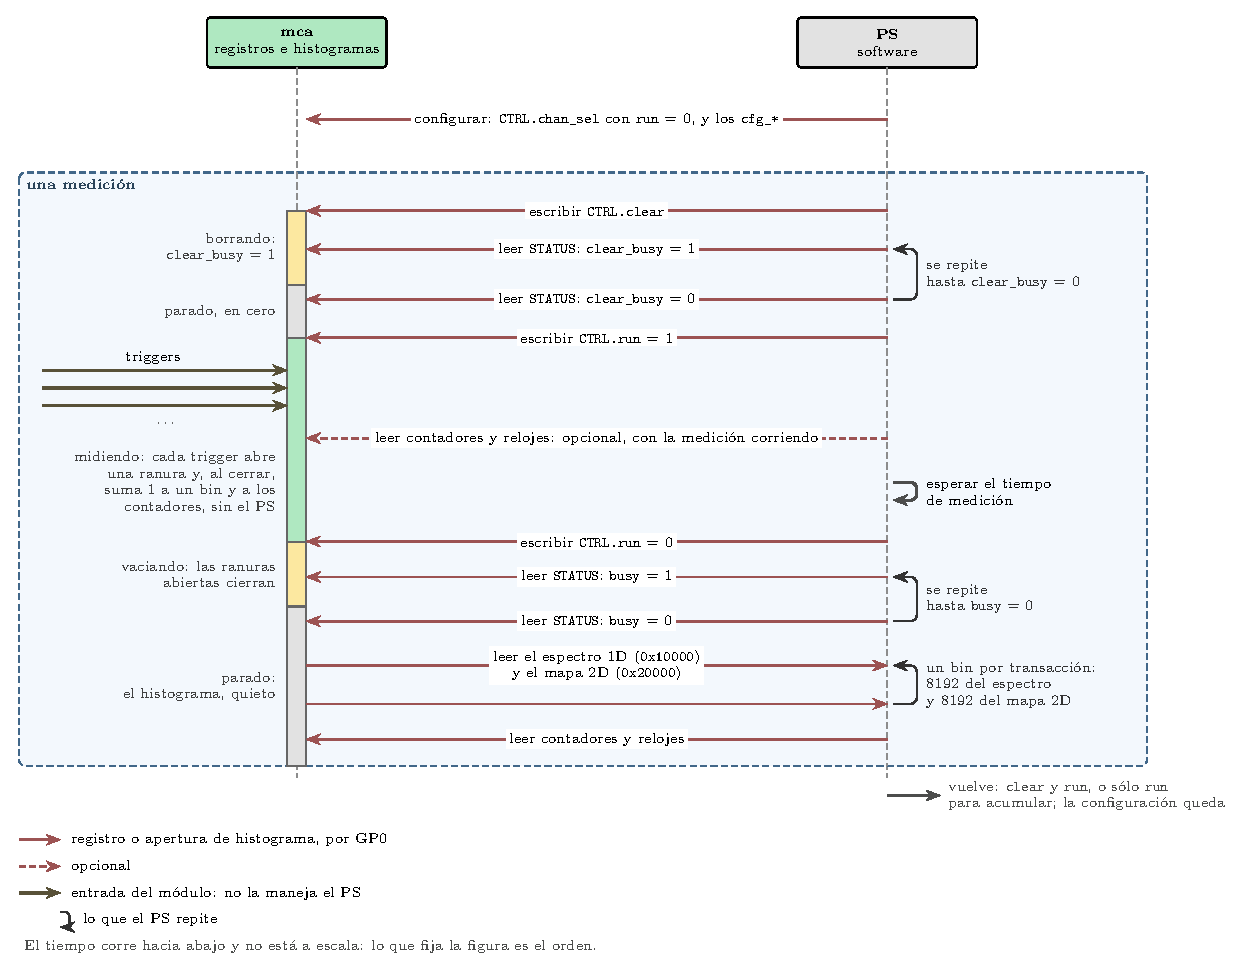
\includegraphics{cap7_secuencia_mca}
\caption[Flujo de utilización del MCA]{%
Flujo de utilización del MCA. Consiste en una fase de configuración y el
lanzamiento de medición.\label{f:implmca-secuencia}}
\end{figure}

Cuando un bin llega al tope ($2^{32}-1$) se levanta la bandera \codigo{full} de
ese histograma (\codigo{full\_1d} o \codigo{full\_2d}), que se mantiene hasta
la próxima limpieza. Por defecto el histograma entero deja de contar, y los
eventos que no entran van a \codigo{cnt\_full\_supp}. Así no hay \emph{overflow} en el
bin, y el espectro no se distorsiona: todos los canales dejan de contar en el
mismo instante, así que sus áreas relativas siguen siendo comparables. Los
relojes, en cambio, siguen corriendo, y la exposición del espectro congelado es
la del instante en que se levantó \codigo{full}. Con
\codigo{cfg\_keep\_full = 1} sólo ese bin queda en el tope y el resto sigue
contando.

%==============================================================================
\section{Vista general del módulo}
\label{S:implmca-vista-general}

En la Fig.~\ref{f:implmca-panorama} se presenta el módulo. La muestra llega con
el canal ya elegido, decimada y retrasada; el retardo compensa la latencia del
disparo del MT, de modo que la ventana abra en el pie del pulso. Los bloques se
agrupan por función, que en la figura se distingue por color. Todo corre en el
reloj del ADC (\qty{125}{\mega\hertz}) y procesa una muestra por ciclo.
\begin{enumerate}
  \item \textbf{Línea de base y conformado} (azul). Actúan sobre toda la señal,
    sin saber dónde hay pulsos: la línea de base \codigo{mca\_baseline}, fija o
    con un seguidor IIR, y el banco de trapecios \codigo{mca\_trap}, tres
    conformados trapezoidales de largos distintos. Se describen en la
    Sec.~\ref{S:implmca-recuperacion}.
  \item \textbf{Segmentación} (amarillo), en \codigo{mca\_window}:
  \begin{enumerate}
    \item Apertura: el flanco de \codigo{trig\_i}. El MCA no detecta pulsos por
      su cuenta: el disparo, y su re-armado, son del MT.
    \item Asignación: el asignador abre la ranura libre de menor índice. Si no
      hay ninguna libre, o si el veto está activo, el disparo se pierde y se
      cuenta (Sec.~\ref{S:implmca-perdidos}).
    \item Cierre: una compuerta fija de \codigo{gate\_long} muestras desde el
      disparo. Cada ranura retiene las compuertas al abrir y cierra sola.
  \end{enumerate}
  \item \textbf{Estadísticos} (verde):
  \begin{enumerate}
    \item Ranuras \codigo{mca\_slot} (\codigo{N\_ACC = 3}): cada una es un juego
      entero de acumuladores. Mientras su ventana está abierta actualizan
      versiones secuenciales de los estimadores: el pico y su instante, las
      cargas $Q_{tot}$ y $Q_{cola}$ y la suma de la meseta de cada forma del
      banco. Al abrir guardan las marcas de solape con otros disparos. Al cerrar
      aplican la ventana de amplitud: si el evento cae afuera, la ranura se
      libera sin publicar.
    \item Divisores \codigo{mca\_div\_restore} (dos, en paralelo): calculan las
      dos \emph{features} de forma, $Q_{cola}/Q_{tot}$ y $\text{pico}/Q_{tot}$, como
      fracciones de 16 bits.
  \end{enumerate}
  \item \textbf{Publicación} (naranja):
  \begin{enumerate}
    \item Publicador \codigo{mca\_publish}: atiende las ranuras cerradas de a
      una, en orden de cierre. Carga los divisores, elige la forma del banco,
      arma el \textbf{bus de \emph{features}} y libera la ranura: 18 ciclos por evento.
      Las ranuras cerradas son la cola de publicación; no hay una FIFO aparte.
    \item Selección de eje y \emph{zoom} \codigo{mca\_zoom}: un mux 16:1 por eje elige
      la \emph{feature}, y el \emph{zoom} la convierte en el índice del bin.
    \item Discriminador \codigo{mca\_discriminator}: acepta o rechaza el evento
      según una \emph{feature} cualquiera del bus.
    \item Histogramas \codigo{mca\_hist} (dos): el espectro 1D y el mapa 2D,
      cada uno en su BRAM, con un incremento por ciclo.
  \end{enumerate}
\end{enumerate}

En gris quedan el banco de registros y la contabilidad: los relojes de 64 bits,
la ocupación de las ranuras y los períodos muertos. Cada bloque se describe en
la Sec.~\ref{S:implmca-submodulos}.

\begin{figure}[H]
\centering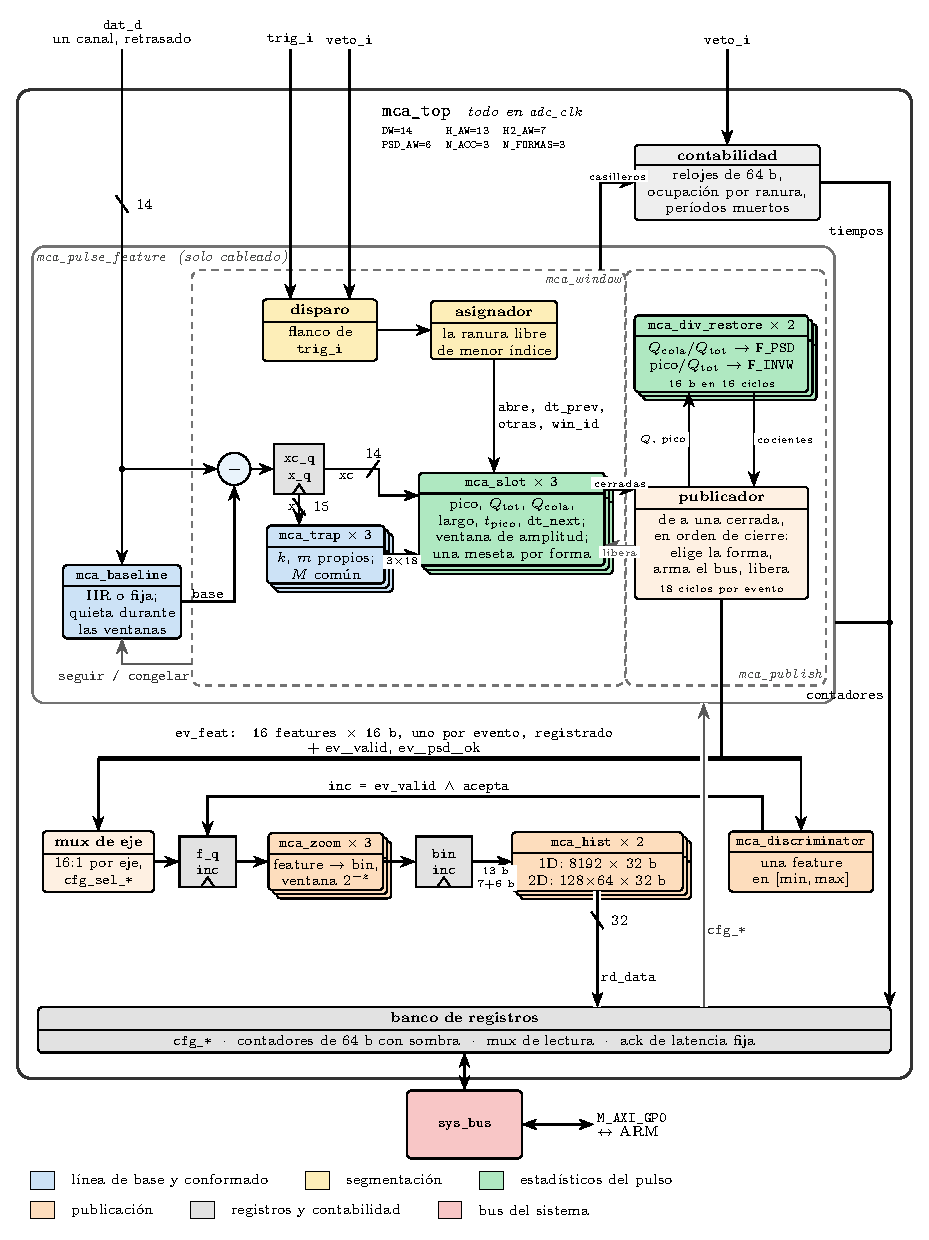
\includegraphics{cap7_panorama_mca}
\caption[Vista general del módulo analizador multicanal]{%
Vista general del módulo analizador multicanal. La muestra entra con el canal
ya elegido, decimada y retrasada, atraviesa \codigo{mca\_pulse\_feature} (la
línea de base, la ventana de medición y la publicación) y cae en el bus de
\emph{features}, del que cuelgan los ejes, el discriminador y los histogramas. El color
indica la función de cada bloque, y los números sobre las flechas son anchos en
bits.\label{f:implmca-panorama}}
\end{figure}

%==============================================================================
\section{Análisis de eventos perdidos}
\label{S:implmca-perdidos}

Seguimos el criterio de la Sec.~\ref{S:osc-tiempo-muerto}: recorremos el
\emph{datapath} y vemos qué hace cada etapa cuando no puede tomar un dato nuevo. Una
etapa \textbf{bloquea} si puede frenar a la anterior, y \textbf{descarta} si su
entrada no tiene \emph{ready} y el dato se pierde. Cada descarte tiene su
contador. En la Fig.~\ref{f:implmca-descarte} se presenta el \emph{datapath} del MCA
desde este punto de vista.

La primera etapa es el disparo, que es externo al MCA: lo genera el MT, y le
corresponde un tiempo de re-armado (Sec.~\ref{S:mt-relanzamiento}). Un pulso que
llega con el disparo desarmado no genera flanco y el MCA no lo ve, así que no
hay cuenta posible: lo que se mide es el tiempo desarmado. Después vienen tres
etapas que descartan y dos que sólo bloquean:
\begin{itemize}
  \item El \textbf{asignador} no puede frenar al disparo. Un disparo que llega
    bajo veto, o sin ranura libre, se pierde.
  \item Las \textbf{ranuras} y el \textbf{publicador} sólo bloquean. Mientras el
    publicador trabaja no libera la ranura que atiende, y las cerradas esperan;
    cuando no queda ninguna libre, el asignador no tiene dónde abrir. Esta
    contrapresión es la que se convierte en tiempo muerto.
  \item Los \textbf{histogramas} no pueden frenar al bus de \emph{features}. Un
    incremento que choca con una lectura del bus o con el barrido de borrado, o
    que llega con el histograma lleno, se pierde.
\end{itemize}

\begin{figure}[H]
\centering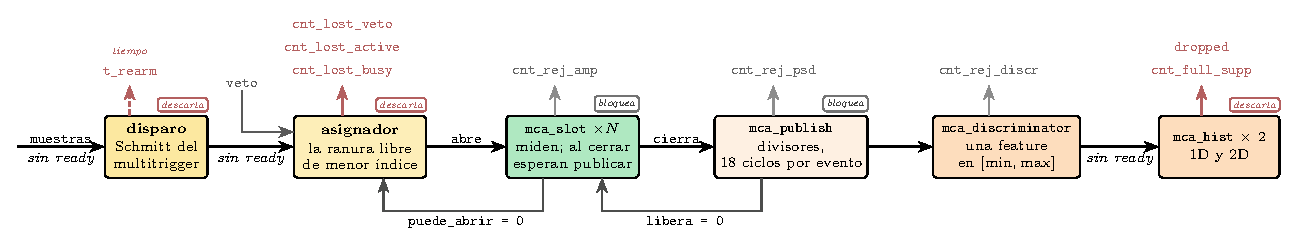
\includegraphics{cap7_freno_descarte}
\caption[\emph{Datapath} del MCA: dónde se frena y dónde se descarta]{%
Entrada por el módulo de multitrigger, \emph{datapath} principal del MCA y los
contadores asociados a cada fase. Las flechas rojas salen de las etapas que
descartan, cada una hacia su contador, y las de vuelta son la contrapresión de
las ranuras y del publicador, que sólo bloquean. Las grises son cortes por
criterio (amplitud, forma y discriminador), que no son tiempo
muerto.\label{f:implmca-descarte}}
\end{figure}

De la Fig.~\ref{f:implmca-descarte} salen dos medidas distintas de lo que se
pierde, y conviene no mezclarlas:
\begin{itemize}
  \item El \textbf{tiempo muerto} es un tiempo: el ancho de las ventanas en que
    la entrada descarta todo lo que llega. Sólo existe a la entrada, porque el
    disparo no se puede frenar: la contrapresión de las etapas que bloquean se
    convierte en tiempo muerto recién ahí. Se mide con relojes, y es lo que
    corrige la exposición del espectro.
  \item Los \textbf{descartes} son una cantidad: los eventos que se pierden en
    cualquier etapa de la cadena, cada uno en el punto en que ocurre. Se miden
    con contadores de eventos, uno por punto de descarte.
\end{itemize}

Las dos medidas sólo se cruzan en el asignador: cada disparo que se pierde ahí
es un descarte que cae dentro de una ventana de tiempo muerto, y por eso la
fracción perdida por el MCA se puede calcular de las dos maneras. En el resto de
la cadena son independientes. El tiempo muerto existe aunque en su ventana no
llegue ningún pulso, y los incrementos que pierde el histograma son descartes
sin tiempo muerto, porque el histograma no frena a nadie y la entrada sigue
abierta. Durante el re-armado del disparo pasa lo contrario: el pulso no genera
flanco, así que no hay descarte que contar y sólo se mide el tiempo. Los
descartes se miden con los contadores que se presentan a continuación, y el
tiempo muerto, con el teselado de la Sec.~\ref{S:implmca-teselado}.

En la Tabla~\ref{t:implmca-contadores} se presentan los contadores del módulo
que no son casilleros del teselado, y lo que representa cada uno. Son de cuatro
tipos: el \textbf{reloj} del barrido de borrado, que queda fuera del teselado;
los de \textbf{períodos}, que resumen los tramos sin ranura libre; los de
\textbf{arribos}, que cuentan disparos, y los de \textbf{incrementos}, que
cuentan eventos que no llegaron al histograma.

\begin{table}[H]
\centering
\caption[Contadores del tiempo muerto y de los eventos perdidos]{%
Contadores del tiempo muerto y de los eventos perdidos, además de los casilleros
del teselado (Tabla~\ref{t:implmca-teselado}) y de la ocupación de las ranuras
(Sec.~\ref{S:ap-mca-ocupacion}). \codigo{t\_clear} y \codigo{max\_dead\_len}
cuentan ciclos de \codigo{adc\_clk}; los demás, eventos. \codigo{cnt\_lost\_busy}
y los \codigo{dropped} de los dos histogramas se leen sumados en un solo
registro, y \codigo{cnt\_lost\_busy} se despeja del balance de
arribos.\label{t:implmca-contadores}}
\small
\begin{tabularx}{\textwidth}{|l|l|>{\raggedright\arraybackslash}X|}
\hline \encabezado \textbf{Tipo} & \textbf{Contador} & \textbf{Qué representa}
  \\ \hline
reloj & \codigo{t\_clear} & los ciclos del barrido de borrado \\ \hline
períodos & \codigo{cnt\_dead\_periods} & los tramos contiguos de ciclos sin
  ranura libre \\
 & \codigo{max\_dead\_len} & el largo del tramo más largo \\
 & \codigo{cnt\_dead\_ext} & los tramos con al menos un disparo adentro
  \\ \hline
arribos & \codigo{cnt\_cross} & los disparos con la adquisición en marcha:
  todos los arribos \\
 & \codigo{cnt\_open} & los disparos que abrieron una ranura \\
 & \codigo{cnt\_lost\_veto} & los disparos perdidos por el veto \\
 & \codigo{cnt\_lost\_active} & los disparos perdidos sin ranura libre, con
  todas midiendo \\
 & \codigo{cnt\_lost\_busy} & los disparos perdidos sin ranura libre, con
  alguna esperando al publicador \\ \hline
incrementos & \codigo{dropped} & los que chocaron con una lectura del bus o con
  el barrido de borrado \\
 & \codigo{cnt\_full\_supp} & los que llegaron con el histograma lleno y
  \codigo{cfg\_keep\_full = 0} \\ \hline
\end{tabularx}
\end{table}

El nombre \codigo{cnt\_cross} viene del MCA1, en el que el arribo era el cruce
del umbral del Schmitt propio (Sec.~\ref{S:ap-mca-mca1}); ahora cuenta
disparos, y el nombre se mantuvo para no cambiar el mapa de registros.

Además de los descartes hay \textbf{rechazos por criterio}: el evento se midió,
pero no cumple una condición configurada (la ventana de amplitud,
\codigo{cnt\_rej\_amp}; una forma inválida, \codigo{cnt\_rej\_psd}; el
discriminador, \codigo{cnt\_rej\_discr}). No son tiempo muerto, y no entran en
la tabla.

Con estos contadores planteamos dos balances. Valen ciclo a ciclo en el
hardware, pero cada lectura del bus tarda unos ciclos y los contadores avanzan
entre una y otra, así que se comprueban con la adquisición parada.
\begin{itemize}
  \item \textbf{Arribos.} Cada disparo con \codigo{run} suma a
    \codigo{cnt\_cross} y a exactamente uno de los contadores de pérdida o a
    \codigo{cnt\_open}, con la misma prioridad que el teselado
    (Sec.~\ref{S:implmca-teselado}): primero el veto y después la causa del
    bloqueo.
    \begin{equation}
      \mathtt{cnt\_cross} = \mathtt{cnt\_open} + \mathtt{cnt\_lost\_veto} +
      \mathtt{cnt\_lost\_active} + \mathtt{cnt\_lost\_busy}
      \label{e:implmca-balance-arribos}
    \end{equation}
  \item \textbf{Eventos.} Con las ranuras vacías (\codigo{busy = 0}), cada
    ventana abierta se cerró y, al cerrar, se publicó o se rechazó por
    amplitud, $\mathtt{cnt\_open} = \mathtt{cnt\_accepted} +
    \mathtt{cnt\_rej\_amp}$. De lo publicado, el espectro 1D cuenta todo salvo
    lo que rechaza el discriminador y lo que ese histograma descarta
    (\codigo{dropped}, \codigo{cnt\_full\_supp}); el 2D descarta además las
    formas inválidas.
\end{itemize}

%==============================================================================
\section{Teselado del tiempo de adquisición}
\label{S:implmca-teselado}

El tiempo muerto es el tiempo en que el sistema no puede procesar un evento
nuevo, y el tiempo vivo es su complemento (Sec.~\ref{S:mca-tiempo-muerto}). En
el MCA, un ciclo es \textbf{vivo} si un pulso que llegara en él abriría una
ranura, y \textbf{muerto} si se perdería. El tiempo vivo, $T_{live}$, es la
exposición del espectro: el tiempo durante el que el módulo pudo registrar
pulsos. Preferimos medirlo, junto con los tiempos muertos, antes que deducirlo
de un modelo. Un modelo supone cómo llegan los pulsos y cuánto dura cada período
muerto, y cualquier diferencia entre esa suposición y la fuente real se vuelve
un error de la corrección, que además crece con la tasa
(Sec.~\ref{S:mca-modelos-tiempo-muerto}).

La dificultad es que un pulso se puede perder por más de una causa, y las causas
se superponen. Se pierde si el veto del escudo del MT está activo, si no hay
ranura libre o si el disparo del MT todavía no se re-armó
(Sec.~\ref{S:mt-relanzamiento}). El veto puede llegar con todas las ranuras
midiendo, y el disparo puede estar desarmado mientras las ranuras están
ocupadas. Si cada causa tuviera su propio contador, un ciclo con dos causas
sumaría en los dos: la suma de los tiempos muertos superaría a
$T_{real} - T_{live}$, y no habría forma de repartir la pérdida entre los
bloques.

Por eso el tiempo de adquisición se \textbf{tesela}: se parte en casilleros que
no se superponen y que entre todos lo cubren, y cada ciclo con \codigo{run} suma
en exactamente uno. Cada casillero es un reloj de 64 bits, y cuando en un ciclo
se cumplen varias condiciones decide una prioridad fija, la del orden de la
Tabla~\ref{t:implmca-teselado}. Así ningún ciclo se cuenta dos veces ni queda
sin contar, el tiempo vivo y el muerto son complementarios por construcción, y
su suma es el tiempo real:
\begin{equation}
  T_{real} = T_{veto} + \underbrace{\mathtt{t\_win} +
  \mathtt{t\_div}}_{\text{muerto del MCA}} +
  \underbrace{\mathtt{t\_rearm}}_{\text{muerto del disparo}} + T_{live}
  \label{e:implmca-teselado}
\end{equation}

\begin{table}[H]
\centering
\caption[Casilleros del teselado del tiempo de adquisición]{%
Casilleros del teselado, en orden de prioridad: cada ciclo con \codigo{run}
suma en el primero cuya condición se cumple. Cuentan ciclos de
\codigo{adc\_clk}; \codigo{realtime}, $T_{real}$, cuenta todos los ciclos con
\codigo{run} y es su suma.\label{t:implmca-teselado}}
\small
\begin{tabularx}{\textwidth}{|l|>{\raggedright\arraybackslash}X|l|}
\hline \encabezado \textbf{Casillero} & \textbf{Suma cuando} &
  \textbf{Tiempo} \\ \hline
\codigo{vetotime} $T_{veto}$ & el veto está activo & excluido \\ \hline
\codigo{t\_win} & no hay ranura libre y todas están midiendo & muerto del MCA
  \\ \hline
\codigo{t\_div} & no hay ranura libre y alguna, ya cerrada, espera al
  publicador & muerto del MCA \\ \hline
\codigo{t\_rearm} & hay alguna ranura libre, pero el disparo del MT no se
  re-armó & muerto del disparo \\ \hline
\codigo{livetime} $T_{live}$ & hay alguna ranura libre y el disparo está
  armado & vivo \\ \hline
\end{tabularx}
\end{table}

La prioridad resuelve las dos superposiciones, y en los dos casos el orden tiene
un motivo:
\begin{itemize}
  \item \textbf{El veto va primero.} Es la convención de la compuerta de un
    MCA: mientras está cerrada, el reloj vivo se para, sea cual sea el estado
    interno. La cola de una ventana que termina bajo veto cuenta como tiempo
    vetado, y no como muerto.
  \item \textbf{El re-armado va después del tiempo muerto del MCA.} Sin ranura
    libre el pulso se pierde igual, esté o no armado el disparo, y si ese ciclo
    sumara también a \codigo{t\_rearm} la pérdida se contaría dos veces.
    \codigo{t\_rearm} es entonces el tiempo muerto que \textbf{agrega} el
    disparo cuando el MCA podía abrir, y \codigo{livetime} queda como lo que un
    pulso ve de verdad: una ranura libre y el disparo armado.
\end{itemize}
\codigo{t\_win} y \codigo{t\_div} no necesitan prioridad entre sí, porque los
distingue si alguna ranura espera al publicador.

\textbf{Por qué se subdivide el tiempo.} Para normalizar el espectro alcanzaría
con dos casilleros, vivo y muerto. Pero cada condición se calcula de forma
independiente, en una etapa distinta de la cadena: el veto en el escudo del MT,
el re-armado en el disparo y la falta de ranura libre en las ranuras del MCA.
Cada casillero representa así un descarte distinto del sistema, y guardarlo es
barato, porque es un contador más. Lo que hay que hacer para achicar cada uno
también es distinto:
\begin{itemize}
  \item \codigo{vetotime} no es tiempo muerto: es tiempo que se excluye a
    propósito, con el escudo del MT, y se descuenta de la exposición y de la
    tasa.
  \item \codigo{t\_rearm} es tiempo muerto del disparo, no del MCA. Se descuenta
    para estimar la tasa, porque en ese lapso ningún pulso genera disparo, y en
    la integración se le atribuye al MT
    (Sec.~\refpend{S:top-tiempo-muerto}{Implementación TOP: «Tiempo muerto por
    módulo», sección que ya no existe en la nota}).
  \item \codigo{t\_win} y \codigo{t\_div} son el tiempo muerto del MCA, pero por
    causas distintas. En \codigo{t\_win} todas las ranuras están midiendo, y
    sólo se achica con más ranuras o con una compuerta más corta. En
    \codigo{t\_div} hay ranuras cerradas que esperan al publicador, y se achica
    publicando más rápido. Con una sola ranura, \codigo{t\_div} es la
    publicación de cada evento; con varias debería ser casi nulo, y si no lo
    es, el cuello de botella es el publicador.
\end{itemize}

Con sólo el tiempo vivo y su complemento no se podría corregir la tasa, ni
saber qué bloque limita. De los casilleros salen los tres tiempos que se
reportan en cada adquisición: el vivo, $T_{live}$; el muerto del MCA,
$\mathtt{t\_win} + \mathtt{t\_div}$, y el del sistema, que le suma
$\mathtt{t\_rearm}$. Sus fracciones se toman sobre el tiempo no vetado,
$T_{real} - T_{veto}$, y con ellas se calculan la tasa de disparos y la fracción
perdida que se presentan al final de esta sección.

Fuera del teselado queda \codigo{t\_clear}, que cuenta los ciclos del barrido de
borrado. Durante el barrido las ranuras siguen midiendo, y lo que se pierde son
incrementos al histograma, que van a \codigo{dropped}: son descartes, y no
tiempo muerto.
\begin{itemize}
  \item \textbf{Tasa de disparos.} Durante el re-armado los pulsos no generan
    disparo, y los que llegan bajo veto se descuentan junto con su tiempo:
    \begin{equation}
      \hat\lambda = f_{clk}\,\frac{\mathtt{cnt\_cross} -
      \mathtt{cnt\_lost\_veto}}{T_{real} - T_{veto} - \mathtt{t\_rearm}}
      \label{e:implmca-lambda}
    \end{equation}
    Esta estimación supone que el disparo está armado mientras el MCA no tiene
    ranura libre. Por la prioridad del teselado, \codigo{t\_rearm} sólo cuenta
    con alguna ranura libre: el re-armado que queda detrás de las ranuras
    ocupadas no se descuenta, y si en ese lapso se pierden pulsos,
    $\hat\lambda$ los subestima.
  \item \textbf{Fracción perdida por el MCA.} Con arribos de Poisson, la
    fracción de pulsos que encuentran al módulo sin ranura libre es la fracción
    del tiempo en que no hay ninguna~\cite{Wolff1982}, y se puede calcular de
    las dos maneras:
    \begin{equation}
      P_{MCA} = \frac{\mathtt{t\_win} + \mathtt{t\_div}}{T_{real} - T_{veto}}
      \simeq \frac{\mathtt{cnt\_lost\_active} +
      \mathtt{cnt\_lost\_busy}}{\mathtt{cnt\_cross} - \mathtt{cnt\_lost\_veto}}
      \label{e:implmca-pmca}
    \end{equation}
    La primera mira el tiempo y la segunda los arribos contados. Con otro
    proceso de arribos, como el de un generador periódico, dejan de coincidir.
\end{itemize}

Los modelos de tiempo muerto, que predicen estos valores a partir de la tasa y
del largo de la ventana, se presentan en la Sec.~\ref{S:ap-mca-modelos}.

%==============================================================================
\section{Métodos de recuperación del pulso}
\label{S:implmca-recuperacion}

El punto de partida de todos los métodos es el disparo de eventos: cada disparo
marca dónde empieza un pulso, y el MCA lo mide en una ventana que arranca ahí.
Cuando dos pulsos se superponen, la ventana de uno contiene parte del otro, y hay
cuatro políticas posibles, que se presentan en la
Tabla~\ref{t:implmca-politicas}.

\begin{table}[H]
\centering
\caption[Políticas para un pulso que se superpone con otro]{%
Políticas para un pulso que se superpone con otro. Las tres primeras procesan cada
evento por separado, a medida que llegan las muestras; la cuarta tiene que
procesar juntos los eventos del par.\label{t:implmca-politicas}}
\small
\begin{tabularx}{\textwidth}{|>{\raggedright\arraybackslash}p{0.17\textwidth}%
  |>{\raggedright\arraybackslash}X|>{\raggedright\arraybackslash}X%
  |>{\raggedright\arraybackslash}X|>{\raggedright\arraybackslash}X|}
\hline \encabezado & \textbf{Sin corrección (1)} & \textbf{Descartar (2)} &
  \textbf{Rescate único (3)} & \textbf{Rescate total (4)} \\ \hline
Qué se hace con un pulso superpuesto & se mide igual, y sale contaminado & se mide
  y se marca, y no llega al histograma & se mide con un estimador que no ve a
  sus vecinos & se mide junto con sus vecinos, y se separan \\ \hline
Eventos publicados por disparo & 1 & 0 o 1 & 1 & 1 \\ \hline
Entrada al cálculo de \emph{features} & flujo de muestras & flujo de muestras & flujo
  de muestras & por transacción: los eventos del par, juntos \\ \hline
En este MCA & la primera versión, el MCA1 & las marcas de solape y el
  discriminador & el banco de trapecios, en \codigo{F\_TRAP} & no se
  implementó \\ \hline
\end{tabularx}
\end{table}

El MCA actual combina la (2) y la (3): todo disparo que encuentra una ranura
libre se mide, las marcas de solape dicen si el resultado está contaminado, y
\codigo{F\_TRAP} usa la forma del banco cuya ventana no alcanza a los vecinos. La
(4) es la descomposición de los estimadores del par: con la distancia entre los
dos pulsos, un sistema lineal de $2 \times 2$ separa sus amplitudes. Se
descartó porque es muy sensible a un error de una muestra en esa distancia, y
porque obliga a retener el primer evento hasta que cierre el segundo.

\subsection{Cálculo secuencial de estimadores}
\label{S:implmca-secuencial}

En los casos (1), (2) y (3) las muestras ingresan al MCA en forma de un flujo, y
simplemente tenemos que actualizar el valor del estadístico de la ventana con
cada muestra nueva, hasta que la ventana termina. Esto se implementa con una
señal de habilitación y simplifica extremadamente el flujo de datos de la
aplicación. El desarrollo matemático formal consiste en poder expresar
$f(x_{i,\ldots, n}) = g( f(x_{i,\ldots, n-1}), x_n)$: no es más que
\textbf{descomponer la aplicación sobre $n$ elementos en los primeros $n-1$ y el
último}; en particular, cuando $f=g$ la operación es asociativa. Ejemplo para la
suma $Q_n$ (integral discreta) y el máximo $A_n$:
\begin{equation}
\begin{aligned}
A_n&= \max_{i=0,\ldots, n} A(x_i) = \max \left( \max_{i=0,\ldots, n-1} A(x_i),
  A(x_n) \right) = \max ( A_{n-1} , A(x_n)) \\
Q_n&= \sum_{i=0,\ldots, n} A(x_i) = \left( \sum_{i=0,\ldots, n-1} A(x_i)
  \right) + A(x_n) = Q_{n-1} + A(x_n)
\end{aligned}
\label{e:implmca-secuencial}
\end{equation}
La aplicación de estas propiedades requiere dos cosas:
\begin{itemize}
  \item \textbf{Un registro por estimador y por ventana abierta}: es lo que
    tiene cada ranura.
  \item \textbf{Arbitrar la publicación}: las ventanas cierran en cualquier
    momento, pero hay un solo publicador, con sus dos divisores, y el histograma
    acepta un incremento por ciclo, porque su BRAM usa un puerto para leer el
    bin y el otro para escribirlo. Por eso las ranuras cerradas esperan su
    turno en una cola.
\end{itemize}

\subsection{Recuperación de la línea de base}
\label{S:implmca-linea-base}

El método más ingenuo de recuperación de la línea de base sería, dada una
ventana completa de un pulso, restarle su media $\bar A$. Esto daría un nuevo
vector de datos compensados, cuyos estadísticos resultan equivalentes a
calcular las siguientes correcciones: $A_{rec} = A - \bar A$, mientras que para
la carga $Q_{rec} = Q - N_{med} \bar A=0$. Igualmente, esto tiene varios
problemas:
\begin{enumerate}
  \item El pulso compensado queda con valor medio 0. Esto está mal, ya que
    muchas de las conformaciones son \textbf{unipolares}, y entonces esto daría
    una desviación sistemática negativa.
  \item No tiene en cuenta que lo que está debajo del pulso cambia a lo largo de
    la ventana. Ahí hay dos cosas distintas: la \textbf{línea de base continua},
    que deriva lentamente, y la \textbf{cola de los pulsos anteriores}, que
    sigue la forma del conformado. Restar una media no corrige ninguna de las
    dos en un estadístico puntual como la amplitud máxima: la primera necesita
    un seguimiento, y la segunda, conocer la forma del pulso.
\end{enumerate}

\subsubsection{Metodologías básicas de recuperación de la línea de base}
\label{S:implmca-lb-basicas}

Las metodologías básicas de recuperación de la línea de base son dos: una
compensación fija, con $b$ = \codigo{cfg\_baseline}, y un seguidor IIR, que
sigue la media de la señal:
\begin{equation}
  b[n] = b[n-1] + 2^{-k}\,\big(v[n] - b[n-1]\big)
  \label{e:implmca-iir}
\end{equation}
Es un pasabajos recursivo de un polo, la media móvil
exponencial~\citecap{Smith1997}{19}. El seguidor es especialmente útil si
tenemos un conformado RC. Se elige una u otra con \codigo{cfg\_bl\_auto}. El
seguidor se queda quieto mientras alguna ranura mide y durante
\codigo{cfg\_bl\_holdoff} muestras después de cada cierre: si siguiera apenas
cierra la compuerta, tomaría la cola y el \emph{undershoot} del pulso como base,
y la arrastraría hacia el lado equivocado.

Estas metodologías se utilizaron en las primeras versiones del sistema y no se
las quitó por dos razones: (1) por su bajo costo y (2) porque son procesamientos
tan generales que no están especializados en ciertas formas de pulsos, como las
que se presentan a continuación.

\subsubsection{Metodologías avanzadas de recuperación de la línea de base}
\label{S:implmca-lb-avanzadas}

Hasta la Sec.~\ref{S:implmca-lb-basicas} teníamos un procesamiento que (1) no tenía en cuenta
la señal de entrada y (2) era un filtro simple. Los métodos avanzados tienen en
cuenta la familia de los pulsos y los disparos. Hay dos familias:
\begin{itemize}
  \item \textbf{Corrección por modelo del pulso}: suponemos que la entrada es la
    superposición de varios pulsos, $f(t) = A(t) + B(t) + C(t) + \ldots$, y a lo
    largo del tiempo estimamos cada uno, $(\hat A(t), \hat B(t), \hat C(t),
    \ldots)$, para restarle a cada medida la cola de los anteriores. Con el
    disparo en $t_0$ hacemos la estimación inicial de $A$, y nuestro
    conocimiento del conformado da el resto del pulso. Necesita un estado por
    pulso, y su error crece con el error en la distancia entre los disparos.
  \item \textbf{Corrección por filtrado}: no se descompone la señal en pulsos.
    Un mismo filtro lineal se aplica a toda la señal, sin saber dónde hay
    pulsos, y convierte cada pulso en una forma de duración finita; dos pulsos
    se pueden medir por separado si esas formas no se pisan, y eso lo deciden
    los disparos. Uno de estos filtros es el conformado trapezoidal. No necesita
    toda la serie del pulso: su salida en cada muestra depende sólo de las
    últimas $2k+m$, y la medida, de unas $k+m$ desde el pie del pulso.
\end{itemize}

Las dos familias están emparentadas: la deconvolución que usa el trapecio,
$y[n] - a\,y[n-1]$, es la extrapolación de la cola con un predictor de una
muestra, aplicada a toda la señal. A continuación describimos la corrección por
filtrado, que es la que implementa el MCA.

\subsection{Utilización de trapecios en el multitrigger y en el MCA}
\label{S:implmca-rapido-lento}

Utilizamos la conformación trapezoidal en dos etapas; esta es la arquitectura
clásica de \textbf{canal rápido y canal lento} (\emph{fast} y \emph{slow
filter}): un filtro corto para saber cuándo y cuántos pulsos hay (el trabajo de
segmentación), y uno largo para determinar los estimadores. En el MCA es el
banco de formas que mide \codigo{F\_TRAP}. En el multitrigger es una fuente de
disparo, \codigo{mt\_pz\_trig}, de un ciclo, mientras que en el MCA se toma la
suma de la meseta en la ventana, \codigo{F\_TRAP}. Los dos usan la misma cuenta
y el mismo \codigo{Mq}.

\subsection{Recuperación por conformación}
\label{S:implmca-trapezoidal}

Esta sección es el análisis del \textbf{canal lento}
(Sec.~\ref{S:implmca-rapido-lento}): el filtro largo que mide la amplitud de
cada pulso, una vez que el canal rápido, el disparo del MT, dijo cuándo llegó y
a qué distancia están sus vecinos.

Si quisiéramos simplemente compensar la cola del conformado, podríamos utilizar
una deconvolución de Jordanov~\cite{Jordanov1994}, que requiere únicamente dos
muestras consecutivas del pulso:
\begin{equation}
  x_d[n] = y[n] - a\,y[n-1], \qquad a = e^{-1/\tau}
  \label{e:implmca-deconv}
\end{equation}
Si $y[n] = A\,e^{-n/\tau}$, el resultado es un impulso de área $A$: la cola
desaparece, y un segundo pulso montado sobre ella mide como si estuviera solo.
El problema es que no promedia el ruido. La amplitud se estima sumando $x_d$ en
unas pocas muestras desde el pie, y esa suma es, en esencia, una muestra después
del pie menos una antes: con ruido blanco $\sigma$ por muestra, su error es
$\approx \sqrt{2}\,\sigma$, sea cual sea el largo de la suma. Mide incluso peor
que el pico, que se compara contra una base promediada sobre miles de muestras.

El conformado trapezoidal de Jordanov y Knoll~\cite{Jordanov1994} resuelve eso
sin perder la compensación de la cola: es la misma deconvolución seguida de dos
sumas móviles, de $k$ y de $l = k+m$ muestras,
\begin{equation}
  H(z) = 16\,(1+M)\,\underbrace{\left(1 - a_M\,z^{-1}\right)}_{\text{deconvolución}}
  \,B_k(z)\,B_l(z), \qquad B_k(z) = \sum_{i=0}^{k-1} z^{-i}, \qquad
  a_M = \frac{M}{1+M}
  \label{e:implmca-trapecio}
\end{equation}
donde $M$ es la constante polo-cero, que se elige para que $a_M = a$
(Sec.~\refpend{S:ap-mca-conformado}{detalles de la conformación
trapezoidal: esa sección de la nota está comentada}). Si $M$ no coincide con la
cola del pulso, la cancelación no es exacta: a la salida queda un resto de la
cola, una exponencial de constante $\tau$ que sigue después del trapecio, y un
pulso que llega encima la suma a su altura. Cuánto pesa un error en $M$ se
presenta en la Sec.~\ref{S:res-polo-cero}. Es \textbf{lineal}, y con una entrada
exponencial $x = A\,e^{-n/\tau}$ la salida tiene tres regiones: una subida de
$k$ muestras, una meseta de $m$ y una bajada de $k$. Se presenta en la
Fig.~\ref{f:implmca-trapecio}. Su largo total es $2k+m$ por larga que sea la
cola de la entrada, y esa huella finita es lo que permite separar pulsos
apilados. La deconvolución sola es el caso $k = 1$, porque $B_1 = 1$: en el
hardware la pregunta no es deconvolución o trapecio, sino qué $k$. En la
Sec.~\refpend{S:ap-mca-conformado}{detalles de la conformación trapezoidal:
esa sección de la nota está comentada} se muestra cómo se obtiene analíticamente
y en HW.

\begin{figure}[H]
\centering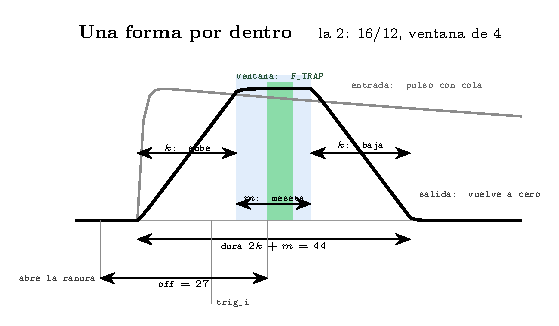
\includegraphics[width=0.6\linewidth]{cap7_trapecio_anatomia}
\caption[Forma básica del conformado trapezoidal]{%
Forma básica del conformado trapezoidal. Consta de una subida de $k$ muestras,
una meseta de $m$ y una bajada del mismo tiempo de subida
$k$.\label{f:implmca-trapecio}}
\end{figure}

La tolerancia al ruido de un conformado trapezoidal depende de $k$. En la
Fig.~\ref{f:implmca-deconv-error} se presentan, contra $k$, dos estadísticos
obtenidos por Monte Carlo: el error relativo de la amplitud de un pulso solo,
que es el ruido de la medición, y la separación mínima a la que el segundo pulso
de un par mide sin sesgo. El ruido baja como $\sigma\sqrt{2/k}$ y la separación
crece como $2k+m$: cuadruplicar $k$ divide el ruido por dos, y cada muestra que
se agrega a $k$ se agrega también a la separación. El punto $k = 1$ es la
deconvolución sola.

\begin{figure}[H]
\centering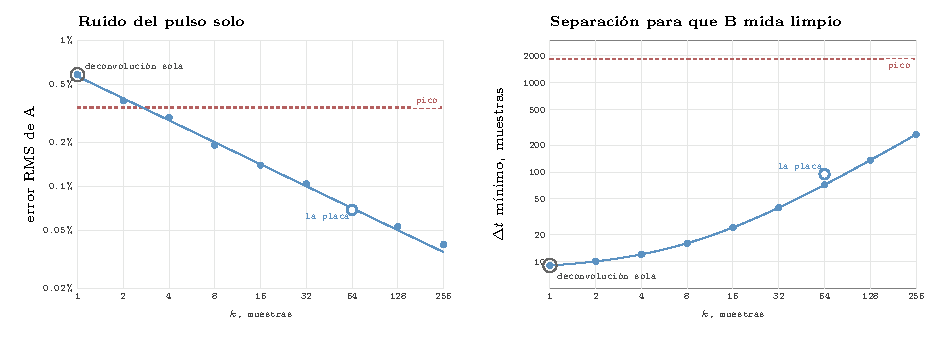
\includegraphics{cap7_trap_deconvolucion}
\caption[Ruido y separación mínima contra $k$]{%
Ruido de la amplitud de un pulso solo (izquierda) y separación mínima para que
el segundo pulso de un par mida sin sesgo (derecha), contra $k$. El punto
$k = 1$ es la deconvolución sola.\label{f:implmca-deconv-error}}
\end{figure}

Además del compromiso entre ruido y separación, el trapecio tiene las siguientes
propiedades:
\begin{itemize}
  \item \textbf{Promedia el ruido.} Pesa con $\approx +1/k$ las $k$ muestras
    después del pie y con $\approx -1/k$ las $k$ de antes: es la diferencia de
    dos promedios de $k$ muestras. Con ruido blanco, es el estimador lineal de
    mínima varianza para la altura de un escalón con ese largo, y su error es
    $\sigma\sqrt{2/k}$. Este efecto se representa en la
    Sec.~\ref{S:res-ruido}.
  \item \textbf{Saca la cola de los pulsos anteriores, pero no la línea de base
    continua.} El término polo-cero convierte cada exponencial en un escalón,
    así que la «base» que se mueve con el apilamiento desaparece de la cuenta.
    Una base continua, en cambio, pasa: un error de base $\varepsilon$ es un
    escalón constante en la entrada, y el trapecio lo deja pasar con ganancia
    $16\,k\,l$. Relativo a la altura de un pulso de amplitud $A$, que es
    $16\,A\,k\,(1+M)$, corre la medida en
    \begin{equation}
      \frac{\Delta A}{A} = \frac{\varepsilon}{A}\,\frac{l}{1+M} \approx
      \frac{\varepsilon}{A}\,\frac{l}{\tau}
      \label{e:implmca-error-base}
    \end{equation}
    Es menos que en el pico, porque $l < \tau$, pero no se cancela. Por eso la
    base se resta antes del trapecio (Sec.~\ref{S:implmca-lb-basicas}).
  \item \textbf{Tolera la pérdida balística y el \emph{jitter} del disparo.} La pérdida
    balística se presenta en la Sec.~\ref{S:mca-tipos-conformado}. El trapecio
    de un pulso real es el ideal convolucionado con su subida, de largo $t_c$:
    las esquinas se redondean y la parte plana de la meseta se achica a
    $\approx m - t_c$. Mientras $m$ supere $t_c$ más la variación del instante
    de disparo, y la ventana de promedio caiga en la parte plana, la altura no
    depende de la subida: no hay déficit balístico. Con $m \le t_c$ no queda
    meseta, y la altura depende de la forma del pulso sin aviso.
  \item \textbf{Es barato.} Dos acumuladores y una multiplicación (el término
    $M$), en enteros, para cualquier $k$ y $m$, más tres líneas de retardo en
    memoria. Uno solo sirve a todas las ranuras.
  \item \textbf{Junto con el canal rápido, dice cuándo midió limpio.} Como la
    huella dura $2k+m$ muestras, el segundo pulso de un par mide limpio si llega
    a más de $\approx k+m$ muestras del primero. Las distancias no las da el
    trapecio sino los disparos del MT, en \codigo{F\_DTPREV} y
    \codigo{F\_DTNEXT} (Sec.~\refpend{S:ap-mca-separacion}{criterio de
    separación: esa sección de la nota está comentada}).
\end{itemize}

\subsection{Utilización del banco de trapecios}
\label{S:implmca-banco}

Para el conformado trapezoidal tenemos un compromiso entre la capacidad de
discernir la separación de pulsos y la precisión de la determinación del
estadístico; este se presenta en la Fig.~\ref{f:implmca-banco-par}. Es
importante notar que no tenemos un conformado por ranura, sino que el
\textbf{tipo de conformado se aplica a toda la señal}. La utilización de un
banco de conformados consiste en aplicar diferentes largos ($k$ y $m$), con la
misma $M$.

\begin{figure}[H]
\centering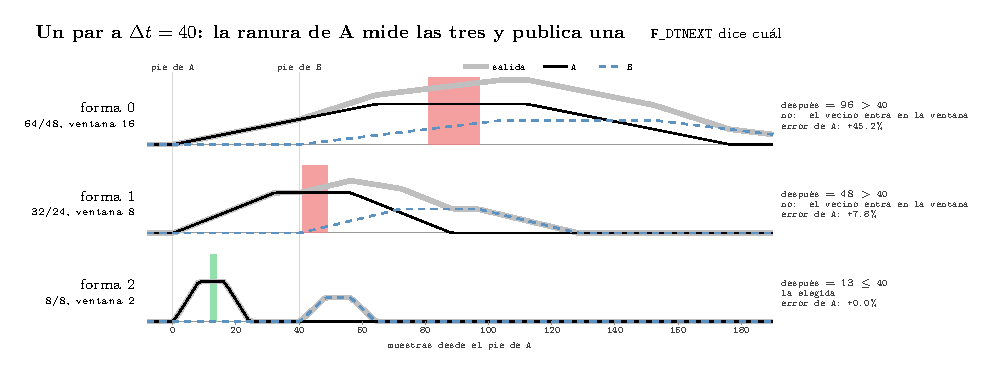
\includegraphics{cap7_banco_formas_par}
\caption[Trapecios de distintas formas sobre un par de pulsos superpuestos]{%
Aplicación de trapecios de forma 64/48, 32/24 y 8/8 para un mismo par de pulsos
superpuestos con $\Delta t=40$. Cada fila es la salida de una forma (gris) con
el aporte de cada pulso por separado, y la ventana en que la ranura de A
promedia la meseta. En las dos formas largas el pulso B entra en esa ventana
(rojo); la 8/8 es la única que queda limpia (verde), y es la que se publica,
porque \codigo{F\_DTNEXT} dice que el vecino está a 40
muestras.\label{f:implmca-banco-par}}
\end{figure}

Es así que, cuando tenemos un disparo, calculamos los elementos para
conformados de diferentes parámetros y, dados los disparos en la ventana,
descartamos los anchos con superposiciones identificadas. La estimación por el
trapecio resulta del \textbf{conformado válido de mayor longitud}. En la
Fig.~\ref{f:implmca-banco-uso} se presenta este mecanismo para conformados de
largo 64/48, 32/24 y 8/8. Para el primer pulso no tenemos ningún otro disparo en
las 97 muestras previas ni en las 96 posteriores al primer disparo P1, de forma
que se decide publicar el primer trapecio (remarcado en azul oscuro). Para el
segundo disparo, P2, hay un disparo durante la ventana posterior del banco
64/48, de forma que se elige el segundo como el mejor. El mismo criterio aplica
para el resto de los disparos.

\begin{figure}[H]
\centering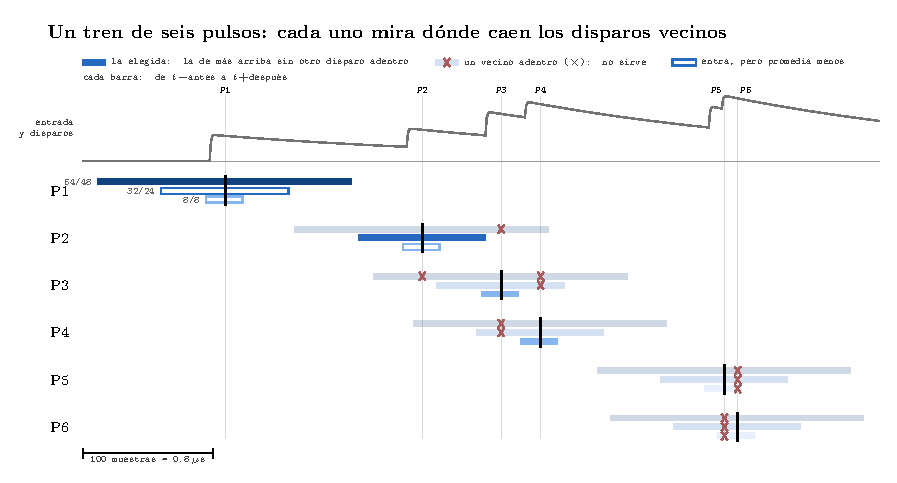
\includegraphics{cap7_banco_uso}
\caption[Esquema de utilización del banco de trapecios]{%
Esquema de utilización del banco de trapecios; cada uno representa un canal
lento de diferente largo. Presentamos los largos 64/48, 32/24 y
8/8.\label{f:implmca-banco-uso}}
\end{figure}

%==============================================================================
\section{Detalles de submódulos}
\label{S:implmca-submodulos}

En esta sección se presentan los detalles de implementación de los submódulos
de la Fig.~\ref{f:implmca-panorama}. Si se quiere ir al \emph{ground truth}, hay
que analizar el RTL de los módulos, en el directorio \ruta{prj/MCA/modulos/mca}
del repositorio del proyecto \incompleto{} (falta el enlace).
\codigo{mca\_pulse\_feature} sólo conecta \codigo{mca\_window} con
\codigo{mca\_publish}, y la línea de base y el banco de trapecios se presentan en
la Sec.~\ref{S:implmca-recuperacion}, así que no tienen subsección propia.

\subsection{Utilización de ranuras y elección de estimadores}
\label{S:implmca-estimadores}

Cada evento se publica con todos sus estimadores a la vez, en un \textbf{bus de
\emph{features}} de 16 posiciones de 16 bits (Fig.~\ref{f:implmca-bus}). El bus es
interno: el ARM no lo ve, y lo que configura es qué posición alimenta cada eje
del histograma y cuál mira el discriminador. Como las posiciones son fijas,
cambiar de estimador no cambia el \emph{bitstream} ni los pulsos medidos: el mismo
pulso puede ir al espectro por su pico y al mapa 2D por su integral y su forma.

Llamamos $x = v - b$ a la muestra $v$ con la línea de base $b$ restada, y
$x_c = \max(x, 0)$ a la misma \textbf{recortada a cero}. Numeramos las muestras
de la ventana desde el disparo, $n = 0$, hasta la compuerta larga $G_l$ =
\codigo{gate\_long}, y contamos sólo las muestras válidas. Las dos cargas son
\begin{equation}
  Q_{tot} = \sum_{n=0}^{G_l-1} x_c[n], \qquad Q_{cola} = \sum_{n=G_s}^{G_l-1}
  x_c[n]
  \label{e:implmca-cargas}
\end{equation}
con $G_s$ = \codigo{gate\_short}, la \textbf{compuerta corta}. $Q_{cola}$ es la
carga que llega después de $G_s$ muestras del disparo, y su fracción de
$Q_{tot}$ mide cuánto pesa la componente lenta del pulso: es el método de
comparación de carga~\cite{Brooks1959}, con el que se distinguen, por ejemplo,
los neutrones de los gammas en un centellador orgánico. Que $G_s$ se cuente
desde el disparo, y no desde el pico, hace a $Q_{cola}$ inmune al \emph{jitter} del
instante del pico. \codigo{F\_TRAP}, en cambio, no suma en toda la ventana sino
en una \textbf{región de la meseta} propia de cada forma del banco: $2^{lw}$
muestras que empiezan \codigo{off} muestras después del disparo, configuradas
por forma con \codigo{cfg\_trap\_off} y \codigo{cfg\_trap\_lw} (se detalla en la
Sec.~\ref{S:implmca-slot}). En la Tabla~\ref{t:implmca-estimadores} se presenta
el procesamiento que recibe cada estimador.

\begin{table}[H]
\centering
\caption[Estimadores del bus de \emph{features}]{%
Estimadores del bus de \emph{features}, agrupados por lo que miden, y el procesamiento
que recibe cada uno. Los tiempos y separaciones se cuentan en muestras válidas.
Los estimadores de solape no miran la señal sino los disparos del MT; cómo se
calculan se detalla en la Sec.~\ref{S:ap-mca-solape}. Las posiciones 11 a 15
del bus están reservadas.\label{t:implmca-estimadores}}
\footnotesize
\begin{tabularx}{\textwidth}{|l|l|>{\raggedright\arraybackslash}p{0.3\textwidth}%
  |>{\raggedright\arraybackslash}X|}
\hline \encabezado \textbf{Tipo} & \textbf{Estimador} & \textbf{Qué representa}
  & \textbf{Procesamiento} \\ \hline
amplitud & \codigo{F\_PEAK} & la altura del pulso en su muestra más alta &
  resta de la línea de base, recorte a cero y máximo de las muestras de la
  ventana \\
 & \codigo{F\_INT} & la carga del pulso, $Q_{tot}$ & resta de la línea de base,
  recorte a cero y suma de todas las muestras de la ventana, corrida
  \codigo{cfg\_q\_shift} bits \\
 & \codigo{F\_TRAP} & la altura del pulso, promediada sobre la meseta del
  trapecio~\cite{Jordanov1994} & resta de la línea de base, conformado
  trapezoidal de cada forma, suma en la región de su meseta corrida $lw$ bits,
  y elección de la forma más larga sin vecinos \\ \hline
forma & \codigo{F\_PSD} & la fracción de la carga en la cola,
  $Q_{cola}/Q_{tot}$ & resta de la línea de base, recorte a cero, suma desde el
  disparo y desde $G_s$, y cociente de las dos \\
 & \codigo{F\_INVW} & el ancho inverso, $\text{pico}/Q_{tot}$: la altura por
  unidad de carga & resta de la línea de base, recorte a cero, máximo y suma de
  la ventana, y cociente de los dos \\ \hline
tiempo & \codigo{F\_LEN} & el largo de la ventana; con la compuerta fija vale
  siempre \codigo{gate\_long} & un contador que arranca en el disparo y suma uno
  por muestra hasta el cierre \\
 & \codigo{F\_TRISE} & el tiempo del disparo al pico & el valor de ese contador
  en la muestra del pico \\ \hline
solape & \codigo{F\_DTPREV} & la separación con el disparo anterior, haya
  abierto ranura o no & un contador común que vuelve a cero con cada disparo,
  leído al abrir la ranura \\
 & \codigo{F\_DTNEXT} & la separación con el siguiente disparo dentro de la
  ventana & el contador de la ventana, leído con el primer disparo que llega
  adentro; \codigo{0xFFFF} si no llega ninguno \\
 & \codigo{F\_SOLAPE} & si había otras ranuras abiertas al abrir, si llegó otro
  disparo adentro y si alguno se perdió & tres marcas en un campo de bits:
  cuántas ranuras había abiertas, \codigo{adentro} y \codigo{perdido} \\
 & \codigo{F\_FORMA} & qué forma del banco se usó en \codigo{F\_TRAP} & el
  índice de la forma elegida; \codigo{0xFFFF} si ninguna cumple \\ \hline
\end{tabularx}
\end{table}

\textbf{Cómo se ubican las compuertas.} Las dos compuertas se configuran juntas,
en muestras desde el disparo (\codigo{cfg\_gate\_len}), y cada ranura las
retiene al abrir. El origen, $n = 0$, es la muestra que llega con el disparo,
retrasada \codigo{cfg\_pre\_dly} muestras: el disparo del MT se produce ya en la
subida del pulso y con la latencia de su filtro, y el retardo corre la ventana
hasta el pie del pulso, así que la carga de la subida entra en $Q_{tot}$. La
compuerta larga fija cuánto mide cada ranura: tiene que cubrir la cola del pulso
hasta que la carga que falta sea despreciable, pero cada muestra de más alarga
el tiempo muerto y la probabilidad de que otro pulso caiga adentro. La compuerta
corta separa la componente rápida de la lenta, así que se pone donde la rápida
ya decayó, y depende del centellador. Las regiones de la meseta de las formas
del banco también tienen que entrar en la compuerta larga, y cada forma tiene un
bit de lectura que avisa si no entra (Sec.~\ref{S:ap-mca-mapa}).

\textbf{Por qué el recorte a cero.} Las \emph{features} de forma son fracciones entre
0 y 1 sólo si todas las muestras que se suman son no negativas: entonces
$0 \le Q_{cola} \le Q_{tot}$ y $\text{pico} \le Q_{tot}$, que es lo que necesita
el divisor, con el numerador menor que el denominador y los dos sin signo. Con
$x$ con signo, una base restada de más, o el \emph{undershoot} de un pulso
anterior al principio de la ventana, pueden hacer negativa, en un pulso chico,
la suma de las primeras $G_s$ muestras, y entonces $Q_{cola} > Q_{tot}$, o
$Q_{tot} \le 0$: el cociente sale de $[0, 1)$ y el evento cae en cualquier lugar
del eje de forma. El recorte tiene un costo. En las muestras de la ventana en
las que la señal está en la base, el ruido deja de promediar a cero, porque sólo
queda su mitad positiva: con ruido gaussiano de desvío $\sigma$, cada una de
esas muestras suma en promedio $E[\max(n, 0)] = \sigma/\sqrt{2\pi} \approx
0.4\,\sigma$. Cuántas muestras de la ventana quedan en el nivel del ruido
depende de la amplitud del pulso, así que el sesgo es mayor en los pulsos
chicos: es una no linealidad de \codigo{F\_INT} cerca de cero. El trapecio usa
$x$ con signo y no tiene este sesgo.

La línea de base también afecta a \codigo{F\_TRAP}: el trapecio deja pasar la
continua, así que un error $\varepsilon$ en la base corre \codigo{F\_TRAP} en una
fracción $\approx \frac{\varepsilon}{A}\,\frac{k+m}{\tau}$ de su altura: menos
que al pico, pero no se cancela. Además del procesamiento de cada estimador, hay
dos filtros que actúan sobre el evento entero, sea cual sea la \emph{feature} que se
histogramea: la ventana de amplitud, que se evalúa al cerrar sobre el pico o
sobre la integral (\codigo{cfg\_amp\_src}), y el discriminador, que mira una
\emph{feature} cualquiera del bus. Por último, cada eje pasa la \emph{feature} que eligió por
su propio \emph{zoom}.

\subsection{Segmentación de eventos:
\texorpdfstring{\texttt{mca\_window}}{mca\_window}}
\label{S:implmca-window}

Es el núcleo de \codigo{mca\_pulse\_feature}: recibe la muestra y el disparo,
decide qué ranura mide cada pulso y lleva la cuenta del tiempo muerto. En la
Fig.~\ref{f:implmca-window} podemos identificar las siguientes regiones:
\begin{enumerate}
  \item \textbf{Disparo} (amarillo): toma el flanco de \codigo{trig\_i} y no el
    nivel, porque un disparo por software dura varios ciclos. Si el flanco cae
    entre dos muestras válidas, espera a la siguiente.
  \item \textbf{Asignador} (amarillo): entre las \codigo{cfg\_n\_acc} primeras
    ranuras, abre la libre de menor índice, si hay una y no hay veto; si no, el
    disparo se pierde y se cuenta. Lo que decide (qué ranura abre y las marcas
    que la ranura guarda al abrir: cuántas había abiertas, \codigo{otras}; la
    distancia al disparo anterior, \codigo{dt\_prev}, y el número de ventana,
    \codigo{win\_id}) se registra en el mismo flanco que la muestra, así que los
    dos llegan a la ranura en el mismo ciclo. La ranura elegida recién figura
    abierta en el ciclo siguiente; \codigo{reserva\_q} la marca ocupada en ese
    ciclo, para que un disparo en la muestra siguiente no elija la misma.
  \item \textbf{Resta de la base} (azul): $x = v - b$ y $x_c = \max(x, 0)$ se
    registran antes de repartirse: $x_c$ va a las ranuras y $x$, con signo, al
    banco de trapecios.
  \item \textbf{Banco de trapecios y región de la meseta} (azul): las tres
    formas corren sobre la misma $x$. Cada forma tiene su propia \textbf{región
    de la meseta}, que es donde se promedia \codigo{F\_TRAP}: empieza
    \codigo{cfg\_trap\_off} muestras después del disparo y dura $2^{lw}$
    muestras (\codigo{cfg\_trap\_lw}). Como el trapecio llega 8 muestras tarde,
    la región se traslada al marco de la ranura, que cuenta desde el disparo:
    $\text{ini} = \text{off} + 8$ y $\text{fin} = \text{ini} + 2^{lw}$. Se
    calcula una sola vez, para todas las ranuras.
  \item \textbf{Umbrales} (verde): los límites de la ventana de amplitud se
    escalan una sola vez, para todas las ranuras.
  \item \textbf{Ranuras} (verde): las \codigo{N\_ACC} instancias de
    \codigo{mca\_slot}, que se describen en la Sec.~\ref{S:implmca-slot}. Nadie
    cierra una ranura desde afuera: cada una cierra sola cuando su largo llega a
    la \codigo{gate\_long} que retuvo al abrir, y vuelve a estar libre cuando el
    publicador la suelta.
  \item \textbf{Hacia la base} (gris): el seguidor de base avanza sólo si
    ninguna ranura mide, ninguna está reservada y no se abre ninguna; cada
    cierre arranca la espera (\emph{holdoff}) de la base.
  \item \textbf{Contabilidad} (gris): en cada ciclo decide si el módulo puede
    abrir y, si no puede, por qué; en cada disparo, a qué contador de arribos
    va, y en cada cierre, si se publicó o se rechazó.
\end{enumerate}

\begin{figure}[H]
\centering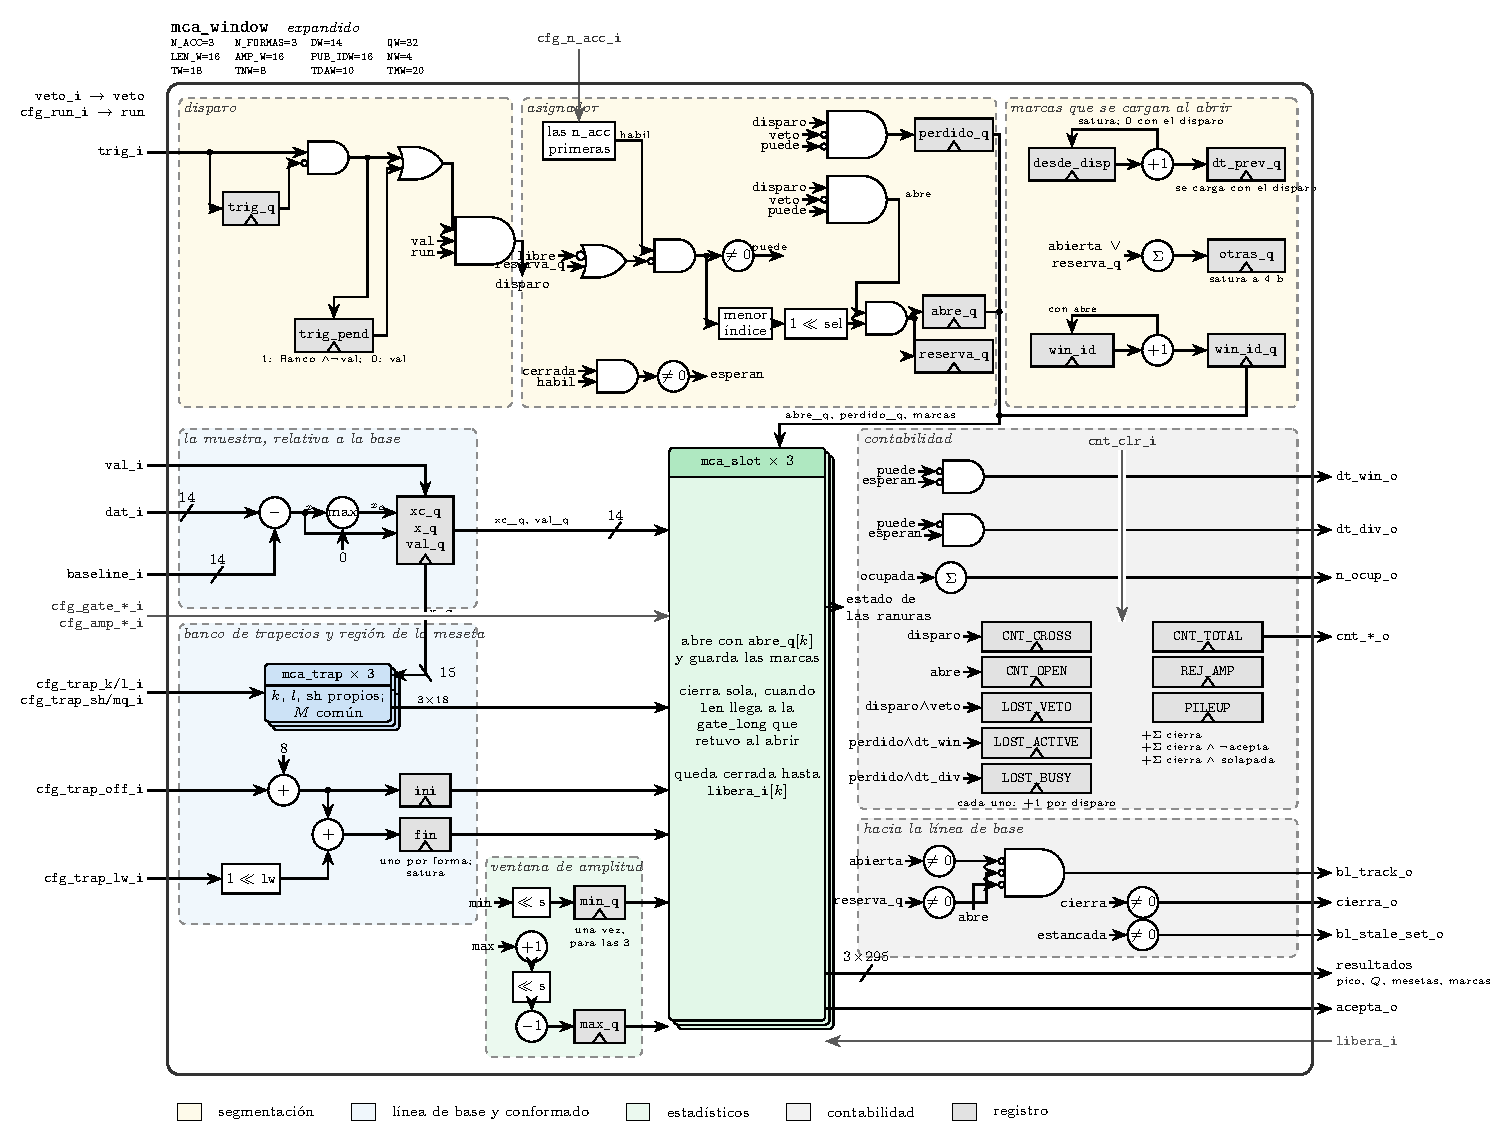
\includegraphics{cap7_panorama_window}
\caption[Vista general de \codigo{mca\_window}]{%
Vista general de \codigo{mca\_window} a nivel de operación. Lo que decide el
asignador se registra en el mismo flanco que la muestra, así que los dos llegan
a la ranura en el mismo ciclo. Ninguna ranura se cierra desde afuera: cada una
cierra cuando su largo llega a la compuerta que retuvo al abrir, y vuelve a
libre cuando el publicador la suelta. A la derecha, la contabilidad.
\codigo{NOMBRE=valor}: parámetros con que lo instancia
\codigo{mca\_pulse\_feature}.\label{f:implmca-window}}
\end{figure}

La contabilidad implementa el \textbf{teselado} de la
Sec.~\ref{S:implmca-teselado}: cada ciclo con \codigo{run} suma en exactamente
un casillero de la Tabla~\ref{t:implmca-teselado}, con la prioridad veto
$>$ \codigo{t\_win} $>$ \codigo{t\_div} $>$ \codigo{t\_rearm} $>$
\codigo{livetime}. Son dos pasos en serie: \codigo{mca\_window} calcula, a
partir del estado de las ranuras, si el módulo puede abrir y, si no puede, por
qué, y \codigo{mca\_top} suma el ciclo al reloj que corresponde. Una ranura
reservada cuenta como ocupada, así que no hay un ciclo en el que el módulo no
pueda abrir y nadie lo cuente.

\subsection{Determinación de estadísticos:
\texorpdfstring{\texttt{mca\_slot}}{mca\_slot}}
\label{S:implmca-slot}

Cada ranura es un juego entero de acumuladores: mide una ventana y, al cerrar,
se queda con el resultado hasta que el publicador lo toma. Así la ranura es a la
vez el lugar donde se mide y un lugar de la cola de publicación. Mientras su
ventana está abierta, actualiza con cada muestra válida las versiones
secuenciales de los estimadores (Sec.~\ref{S:implmca-recuperacion}). En la
Fig.~\ref{f:implmca-slot} se presenta con una fila por acumulador:
\begin{enumerate}
  \item \textbf{Compuertas} (amarillo): al abrir retiene \codigo{gate\_short} y
    \codigo{gate\_long}, así que una ventana mide con lo que se configuró cuando
    abrió, aunque se cambie a mitad de una corrida. \codigo{len} cuenta las
    muestras desde el disparo, y la ranura cierra cuando llega a
    \codigo{gate\_long}. Al cerrar, si la amplitud está dentro de la ventana,
    guarda el resultado hasta que el publicador la libera; si no, se libera sin
    publicar.
  \item \textbf{Pico} (verde): $x_c > \text{pico}$, con comparación estricta: en
    un techo plano gana la primera ocurrencia. Con $\ge$ el instante del pico se
    correría al final de la meseta, y el tiempo al pico saldría arbitrariamente
    largo.
  \item \textbf{Ventana de amplitud} (verde): compara la amplitud, el pico o la
    integral, contra $[\min, \max]$. Se evalúa un ciclo antes del cierre, con
    las restas llevadas en registros sombra, para sacarla del camino crítico.
  \item \textbf{Cargas} (verde): $Q_{tot}$ suma $x_c$ desde la muestra del
    disparo, y $Q_{cola}$ desde la muestra \codigo{gate\_short}, las dos hasta
    el cierre. Al abrir, $Q_{tot}$ arranca con la muestra del disparo y
    $Q_{cola}$ en cero.
  \item \textbf{Meseta, una por forma} (verde): suma la salida del trapecio de
    cada forma mientras la muestra está dentro de la región de su meseta,
    $\text{ini} \le \text{\codigo{len}} < \text{fin}$, y cuenta cuántas sumó. El
    publicador divide esa suma por $2^{lw}$, con un corrimiento de $lw$ bits, y
    obtiene \codigo{F\_TRAP}. Si la cuenta no llegó a $2^{lw}$, porque la
    compuerta cerró antes de terminar la región, publica cero en vez de un
    promedio parcial, que caería en cualquier lugar del espectro: el cero cae en
    el canal 0, donde se ve.
  \item \textbf{Marcas de solape} (gris): \codigo{otras}, \codigo{dt\_prev} y
    \codigo{win\_id} se cargan al abrir. Si llega otro disparo dentro de la
    ventana, se marca \codigo{adentro}, el primero fija \codigo{dt\_next}, y si
    no encontró ranura libre se marca \codigo{perdido}. La ranura no corrige
    nada: deja escrito en el resultado que midió sobre otro pulso.
  \item \textbf{Amplitud} (verde): la integral, $Q_{tot}$ corrida
    \codigo{cfg\_q\_shift} bits y saturada a 16, y la amplitud elegida para la
    ventana, el pico o esa integral.
\end{enumerate}

\begin{figure}[H]
\centering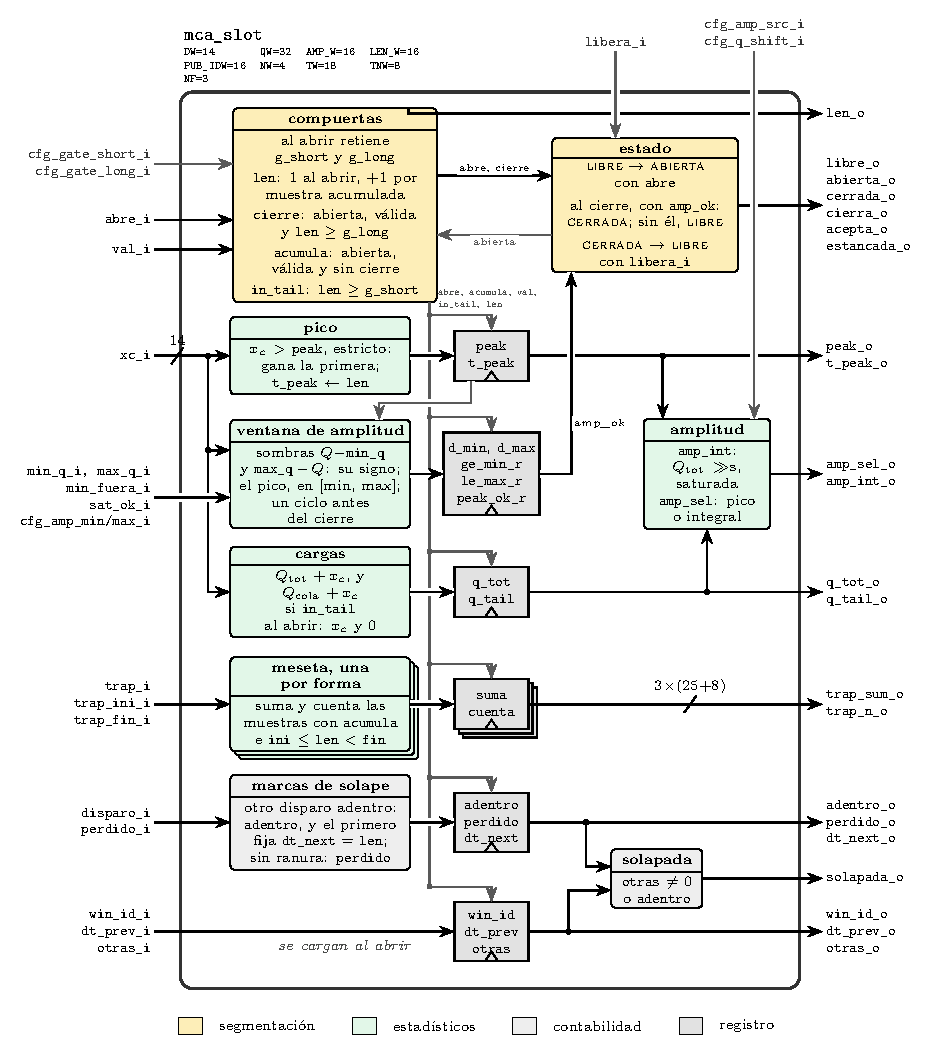
\includegraphics{cap7_panorama_slot}
\caption[Vista general de \codigo{mca\_slot}]{%
Vista general de \codigo{mca\_slot}. Arriba, el control; abajo, una fila por
acumulador: la lógica calcula el valor siguiente y el control elige entre ese,
el de apertura y el que ya tenía. Las marcas de solape no corrigen nada: dejan
escrito en el resultado que se midió sobre otro pulso. \codigo{NOMBRE=valor}:
parámetros con que la instancia \codigo{mca\_window}.\label{f:implmca-slot}}
\end{figure}

Cada ranura suma la meseta de todas las formas del banco en paralelo, porque la
forma recién se puede elegir al cerrar, cuando ya se sabe si llegó otro disparo
dentro de la ventana. En la Fig.~\ref{f:implmca-meseta} se presenta un par de
pulsos visto desde la ranura del primero: la ventana de la forma más corta
termina antes de que llegue el segundo, y en ese momento todavía no se sabe si
las ventanas largas van a quedar limpias.

\begin{figure}[H]
\centering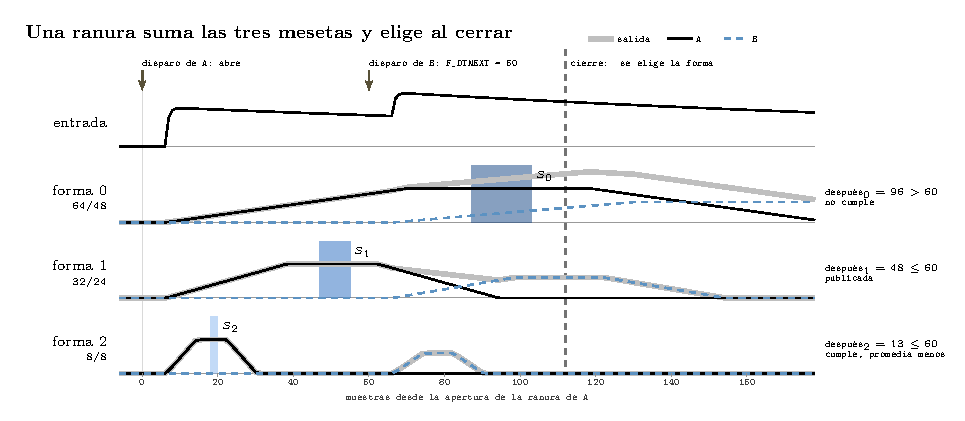
\includegraphics{cap7_meseta_ranura}
\caption[Un par de pulsos visto desde la ranura del primero]{%
Un par de pulsos a 60 muestras visto desde la ranura de A. Hay un trapecio por
forma para toda la señal, y la ranura suma cada uno sobre su ventana ($S_0$ a
$S_2$) mientras su compuerta está abierta. \codigo{F\_DTNEXT} recién es
definitivo al cerrar, y ahí se elige: la 64/48 no cumple, y de las dos que
cumplen se publica la más larga.\label{f:implmca-meseta}}
\end{figure}

\subsection{Publicación a histograma:
\texorpdfstring{\texttt{mca\_publish}}{mca\_publish}}
\label{S:implmca-publish}

El publicador atiende las ranuras cerradas de a una, en el orden en que
cerraron. Los datos del evento no se copian: quedan en su ranura, que no vuelve
a abrir hasta que el publicador la libera. Lo único que hay que guardar es el
orden, y para eso está la \textbf{cola de índices}, una FIFO de
\codigo{N\_ACC} lugares en la que cada lugar tiene el número de una ranura
cerrada. Cuando una ranura cierra, su número entra al final de la cola; si
cierran varias en el mismo ciclo, entran por orden de índice. Cuando el
publicador termina un evento, sale la cabeza y las demás avanzan un lugar. La
cola no puede desbordar, porque cada ranura está en ella a lo sumo una vez. Por
cada evento:
\begin{enumerate}
  \item Guarda en \codigo{cur} el número de la cabeza de la cola y arranca los
    dos divisores, que toman sus operandos de esa ranura. Si la cola estaba
    vacía y el publicador libre, arranca con la ranura que cierra, en el mismo
    flanco del cierre.
  \item En el ciclo en que los divisores toman los operandos, elige la forma
    del banco que se publica en \codigo{F\_TRAP}, así que la elección no agrega
    latencia.
  \item Cuando terminan, carga en un solo flanco las 16 posiciones del bus de
    \emph{features}, lo marca válido durante un ciclo (\codigo{ev\_valid}) y libera la
    ranura.
\end{enumerate}

Cada evento tarda 18 ciclos: el del arranque, el de carga, las 16 iteraciones de
los divisores y el de salida. La latencia no depende del evento, así que el
tiempo que agrega el publicador es siempre el mismo.

La elección de la forma se presenta en la Fig.~\ref{f:implmca-eleccion-forma}.
Por cada forma $f$ (tipo de trapecio en el banco), dos comparaciones dicen si su
ventana queda libre de vecinos: el disparo anterior tiene que estar al menos
$\text{antes}_f$ muestras atrás y el siguiente, al menos $\text{después}_f$
muestras adelante. Entre las formas que cumplen, una prioridad toma la primera,
de la más larga a la más corta, y su suma, dividida por el largo de su ventana,
es \codigo{F\_TRAP}; su índice va a \codigo{F\_FORMA}. Si ninguna cumple, el
pulso queda marcado, con \codigo{F\_TRAP} en cero.

\begin{figure}[H]
\centering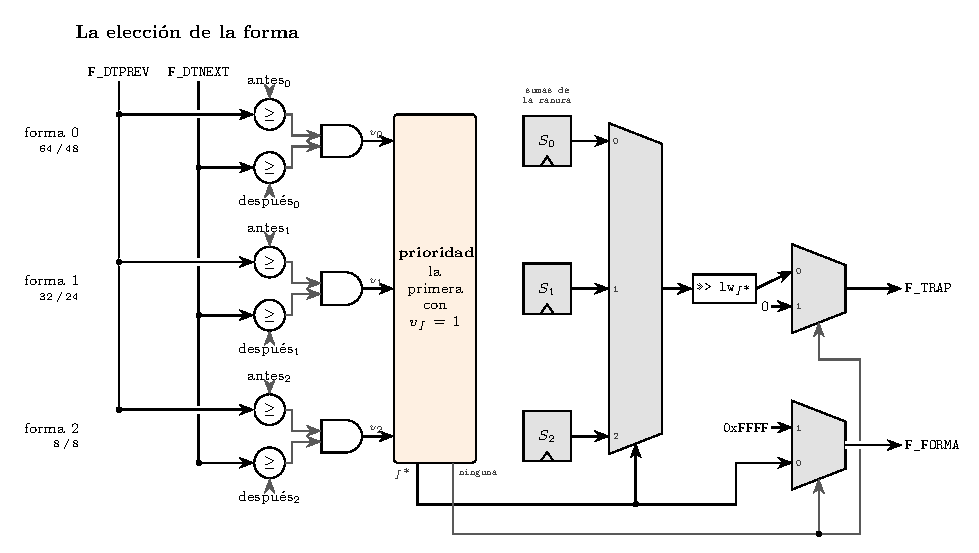
\includegraphics[width=0.75\linewidth]{cap7_eleccion_forma}
\caption[Elección de la forma del banco]{%
La elección de la forma. Por forma, dos comparaciones contra sus umbrales y una
Y; la prioridad toma la primera válida y su índice elige la suma, que el
corrimiento convierte en el promedio sobre la meseta. Si ninguna es válida,
\codigo{F\_TRAP} = 0 y \codigo{F\_FORMA} =
\codigo{0xFFFF}.\label{f:implmca-eleccion-forma}}
\end{figure}

En la Fig.~\ref{f:implmca-bus} se presenta cómo se arma el bus: el resultado de
la ranura que se publica, los cocientes de los divisores y la forma elegida, y
quién lo consume en \codigo{mca\_top}.

\begin{figure}[H]
\centering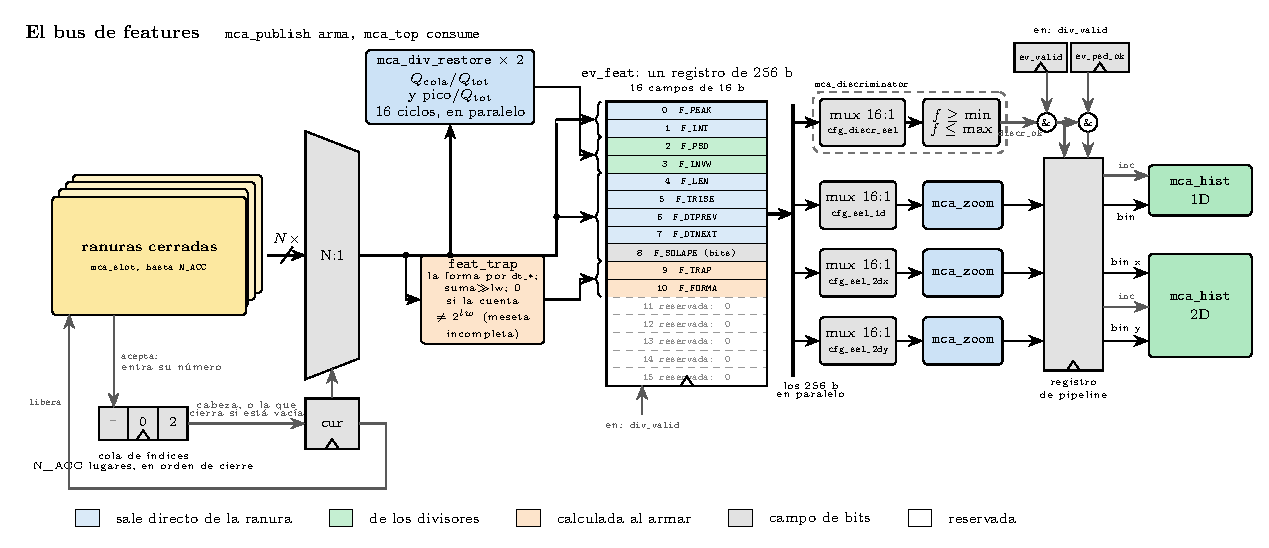
\includegraphics{cap7_bus_features}
\caption[Bus de \emph{features}]{%
Bus de \emph{features}. Cada ranura cerrada guarda su resultado hasta que el publicador
la libera, y la cola de índices guarda el orden en que cerraron (en el ejemplo,
la 2 y después la 0). \codigo{ev\_feat} es un único registro de 256 bits, 16
posiciones de 16 bits que se cargan en el mismo flanco que \codigo{ev\_valid} y
\codigo{ev\_psd\_ok}, así que todo lo que sale es del mismo evento. Las 16
posiciones salen en paralelo, y cada consumidor elige la suya con su propio
multiplexor 16:1, el discriminador incluido.\label{f:implmca-bus}}
\end{figure}

\subsection{Divisor restaurador:
\texorpdfstring{\texttt{mca\_div\_restore}}{mca\_div\_restore}}
\label{S:implmca-div}

Las dos \emph{features} de forma, $Q_{cola}/Q_{tot}$ y $\text{pico}/Q_{tot}$, se
calculan con dos \textbf{divisores restauradores}. Las dos son fracciones entre
0 y 1, y el divisor las entrega como un entero de 16 bits:
\begin{equation}
  q = \left\lfloor \frac{\text{num}}{\text{den}}\, 2^{16} \right\rfloor, \qquad
  \text{num} < \text{den}
  \label{e:implmca-divisor}
\end{equation}
Numerador y denominador son enteros sin signo de 32 bits, tal como salen de la
ranura, y el cociente es una fracción en punto fijo con 16 bits fraccionarios y
sin parte entera (Q0.16): una fracción de 0.5 sale como $2^{15}$, y el cociente
ocupa directamente el rango completo del bus. El divisor restaurador es la
división larga en binario~\citecap{Parhami2010}{13}: saca un bit del cociente
por ciclo, con una comparación y una resta y sin multiplicadores, así que los 16
bits salen en 16 ciclos, sea cual sea el ancho de los operandos.

Los dos divisores trabajan en paralelo, uno por \emph{feature}. Comparten el
denominador $Q_{tot}$ y el arranque, así que el segundo no agrega tiempo. La
latencia es fija, incluso en los casos borde, y eso es deliberado: hace que el
tiempo que tarda el publicador por evento sea siempre el mismo, y con él el
tiempo muerto que agrega. Dividimos $\text{pico}/Q_{tot}$ y no al revés porque
el divisor exige un numerador menor que el denominador, y
$Q_{tot} = \sum x_c \ge \max x_c$ siempre, gracias al recorte a cero.

Los casos borde se tratan aparte. Con $Q_{tot} = 0$ el cociente saldría con
todos los bits en uno, y con $\text{num} \ge \text{den}$ no entraría en 16 bits:
con $\text{num} = \text{den}$, por ejemplo, daría $2^{16}$, que se envuelve a
cero. En los dos casos el evento caería en un extremo del eje sin aviso. En
lugar de eso, si $Q_{tot} = 0$ o $Q_{cola} \ge Q_{tot}$, la forma se marca como
inválida (\codigo{cnt\_rej\_psd}): el evento entra al 1D, pero no al 2D. El
ancho inverso sólo llega a 1 con un pulso de una sola muestra, y en ese caso
satura en \codigo{0xFFFF}.

\subsection{Módulo de \emph{zoom}:
\texorpdfstring{\texttt{mca\_zoom}}{mca\_zoom}}
\label{S:implmca-zoom}

Antes del \emph{zoom}, un mux 16:1 por eje elige qué \emph{feature} del bus va a ese eje
(\codigo{cfg\_sel\_1d}, \codigo{cfg\_sel\_2dx} y \codigo{cfg\_sel\_2dy}), con la
numeración de la Tabla~\ref{t:implmca-estimadores}. El \emph{zoom} le asigna a esa
\emph{feature} el índice del bin. La ventana del eje es
$\left[k\,2^{16-z},\ (k+1)\,2^{16-z}\right)$, con $z$ el nivel de \emph{zoom} y $k$ el
índice de la ventana, $0 \le k < 2^z$, como se presenta en la
Fig.~\ref{f:implmca-zoom}. Con $z = 0$, que es el valor de \emph{reset}, la ventana es
el rango completo de la \emph{feature}, y el bin son sus bits más altos. La ventana
empieza en un múltiplo de su ancho, y su ancho es una potencia de dos. Así la
cuenta es sólo de bits: la \emph{feature} está adentro si sus $z$ bits más altos valen
$k$, y el bin son los bits siguientes, sin restar ni multiplicar. Además, los
bins de un nivel son subdivisiones exactas de los del anterior: un bin de nivel
$z$ es la suma de dos de nivel $z+1$. Por eso espectros tomados con \emph{zoom}
distinto se combinan sumando enteros, sin re-muestrear.

Un evento fuera de la ventana satura: va al último bin si está por encima y al
primero si está por debajo, así que los bins de los extremos avisan del
desborde. El \emph{zoom} no mejora la resolución: sólo achica la pérdida por bineado
(Sec.~\ref{S:implmca-fisher-bineado}). Sirve para ubicar el eje sobre una región
de interés y para poder usar un histograma más chico.

\begin{figure}[H]
\centering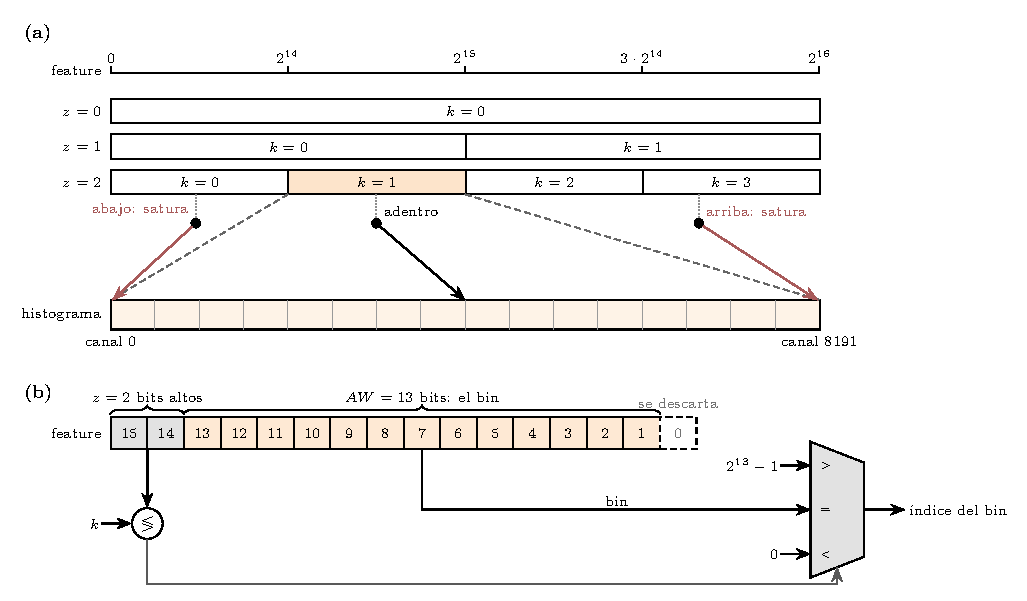
\includegraphics{cap7_zoom_ventanas}
\caption[El \emph{zoom} de un eje del histograma]{%
El \emph{zoom} de un eje, para el espectro 1D (\emph{feature} de 16 bits, 8192 canales). (a)
En el nivel $z$ el rango de la \emph{feature} se parte en $2^z$ ventanas iguales y
alineadas, y la ventana $k$ ocupa el histograma entero. Con $z = 2$ y $k = 1$,
un evento adentro cae en el bin proporcional, y los de afuera saturan en el
primer y en el último canal. (b) La misma cuenta en bits: los $z$ bits altos se
comparan con $k$, los 13 siguientes son el bin y el resto se
descarta.\label{f:implmca-zoom}}
\end{figure}

\subsection{Discriminador:
\texorpdfstring{\texttt{mca\_discriminator}}{mca\_discriminator}}
\label{S:implmca-discr}

Acepta o rechaza el evento según una \emph{feature} del bus, elegida con
\codigo{cfg\_discr\_sel}. Con \codigo{cfg\_discr\_out = 0} acepta si la \emph{feature}
está en $[\min, \max]$, y con \codigo{cfg\_discr\_out = 1}, si está afuera;
deshabilitado, acepta todo. Con $\min > \max$ el intervalo es vacío, así que
rechaza todo o acepta todo, según el modo. Un evento rechazado no va a ninguno
de los dos histogramas y se cuenta en \codigo{cnt\_rej\_discr}.

Está después de los divisores para que pueda mirar las \emph{features} de forma, que no
existen hasta que el divisor termina: un corte en $\text{pico}/Q_{tot}$ separa
los pulsos apilados, que son más anchos, de los limpios. El costo es que todo
evento paga la latencia del publicador antes de poder ser rechazado.

\subsection{Módulo de histograma:
\texorpdfstring{\texttt{mca\_hist}}{mca\_hist}}
\label{S:implmca-hist}

Cada histograma es una memoria de $2^{AW}$ contadores de 32 bits, en una BRAM de
doble puerto simple: un puerto sólo escribe y el otro sólo lee. El 1D tiene 8192
canales y el 2D, $128 \times 64$ bines. Un incremento es una lectura, una suma y
una escritura en tres etapas: en el ciclo $m$ lee el bin, en $m+1$ calcula el
valor nuevo y en $m+2$ lo escribe. Con la lectura y la escritura en puertos
distintos acepta un incremento por ciclo. Si dos eventos seguidos caen en el
mismo bin, el segundo leería un valor viejo; por eso el valor se toma
directamente de las dos escrituras en vuelo (\emph{forwarding}) cuando la
dirección coincide.
\begin{itemize}
  \item \textbf{Lectura del bus}: tiene prioridad sobre el incremento en el
    puerto de lectura. Un incremento que llega en ese ciclo se pierde y se
    cuenta en \codigo{dropped}.
  \item \textbf{Borrado}: un barrido de $2^{AW}$ ciclos que usa sólo el puerto
    de escritura, así que el bus puede seguir leyendo mientras se borra. Los
    incrementos que llegan durante el barrido también van a \codigo{dropped}, y
    los que estaban en vuelo se descartan, para no dejar cuentas en un
    histograma recién borrado.
  \item \textbf{Lleno}: los contadores saturan en $2^{32} - 1$. El primer bin
    que llega al tope levanta \codigo{full}, que queda hasta el próximo borrado;
    con \codigo{cfg\_keep\_full = 0} se congela el histograma entero y los
    incrementos siguientes van a \codigo{cnt\_full\_supp}
    (Sec.~\ref{S:implmca-flujo}).
\end{itemize}

% Bibliografía de este capítulo. Va al final del archivo, siempre.
\bibliografiacapitulo

%%% Local Variables:
%%% mode: latex
%%% TeX-master: "template"
%%% End:
